%%%%%%%%%%%%%%%%%%%%%%%%%%%%%%%%%%%%%%%%%%%%%%%%%%%%%%%%%%%%%%%%%%%%%%%%%%% 
% 
% Generic template for TFC/TFM/TFG/Tesis
% 
% By:
% + Javier Macías-Guarasa. 
% Departamento de Electrónica
% Universidad de Alcalá
% + Roberto Barra-Chicote. 
% Departamento de Ingeniería Electrónica
% Universidad Politécnica de Madrid   
% 
% Based on original sources by Roberto Barra, Manuel Ocaña, Jesús Nuevo,
% Pedro Revenga, Fernando Herránz and Noelia Hernández. Thanks a lot to
% all of them, and to the many anonymous contributors found (thanks to
% google) that provided help in setting all this up.
% 
% See also the additionalContributors.txt file to check the name of
% additional contributors to this work.
% 
% If you think you can add pieces of relevant/useful examples,
% improvements, please contact us at (macias@depeca.uah.es)
% 
% You can freely use this template and please contribute with
% comments or suggestions!!!
% 
%%%%%%%%%%%%%%%%%%%%%%%%%%%%%%%%%%%%%%%%%%%%%%%%%%%%%%%%%%%%%%%%%%%%%%%%%%% 

\chapter{SmartMOT: Exploiting the fusion of HD maps and Multi-Object Tracking for Real-Time scene understanding}
\label{cha:smartmot_exploiting_the_fusion_of_hdmaps_and_mot}

\begin{FraseCelebre}
	\begin{Frase}
		Avanzad, sin temor a la oscuridad. \\
		Luchad jinetes de Theoden. \\
		Caerán las lanzas, se quebrarán los escudos. \\
		Aún restará la espada. \\
		Rojo será el día, hasta el nacer del sol. \\
		Cabalgad, cabalgad, cabalgad hacia la desolación \\ 
		y el fin del mundo. Muerte, muerte, muerte.
	\end{Frase}
	\begin{Fuente}
		Discurso de Theoden, Rey de Rohan \\
		El Señor de los Anillos: El Retorno del Rey
	\end{Fuente}
\end{FraseCelebre}

\section{Introduction}
\label{sec:4_introduction}

In order to achieve a reliable navigation, \acp{ADS} must perform safe driving behaviours following conventional traffic rules. In that sense, the perception layer represents one of the most important modules of an Autonomous Driving (AD) stack, responsible of analyzing the online information, also referred as the traffic situation, through the use of a global perception system \cite{gomez2019simulating} which involves different on-board sensors as: Light Detection And Ranging (LiDAR), Inertial Measurement Unit (IMU) , RAdio Detection And Ranging (RADAR), Differential-Global Navigation Satellite System (D-GNSS), Wheel odometers or Cameras.

One of the key concepts when developing safe \acp{ADS} is the perception of the environment. Furthermore, the reliability of a Collision Avoidance System (CAS) lies on the performance of the environment detector and its ability to predict future situations. In that sense, a real-time \ac{MOT} system, which goal is to associate detections (usually in the 3D or \ac{BEV} space) in a sequence, is essential for \ac{AD} applications, representing in most cases the preliminary stage before predicting the subsequent future trajectories of these obstacles in the scene, giving the car a valuable reaction time to avoid critical situations or to anticipate its behaviour for the corresponding traffic scenario. The improvements in object detection in the last years have allowed the research community, specially those groups related to \ac{AD}, to focus on \ac{MOT} techniques as a preliminary stage before implementing \ac{MP}, yielding higher accuracy at the cost of computational cost and complexity, making its use prohibitive in real-time systems. 

\ac{MOT} systems aim to estimate the orientation, location and scale of all the objects in the environment over time. While object detection only captures the information of the environment in a single frame, a tracking system must take temporal information into account, filtering outliers (\aka false positives) in consecutive detections and being robust to partial or full occlusions. When travelling throughout a route programmed by the path-planner, the vehicle may detect an undetermined number of unforeseen objects over which the \ac{MOT} module should consider only the most relevant from a safety point of view (such as pedestrians, cyclists or cars) to predict and monitor their trajectories. Then, the vehicle can use the evolution of the scene over time to infer driving behaviour and motion patters for improved \ac{MP}.

Most \ac{MOT} approaches \cite{weng20203d, chiu2021probabilistic} model the state of each obstacle with its 3D position, scale, orientation and their corresponding linear and angular velocity. These approaches introduce an unnecessary complexity and computational cost to the system since most traffic scenes can be described in terms of 2D position, angular and linear velocity, apart from the orientation and scale of the resulting bounding box, that is, a \ac{BEV} perspective, as depicted in Figure \ref{fig:chapter_4_SmartMOT/ITSC_2020_coordinates_conversion}. 

\begin{figure}[h]
	\centering
	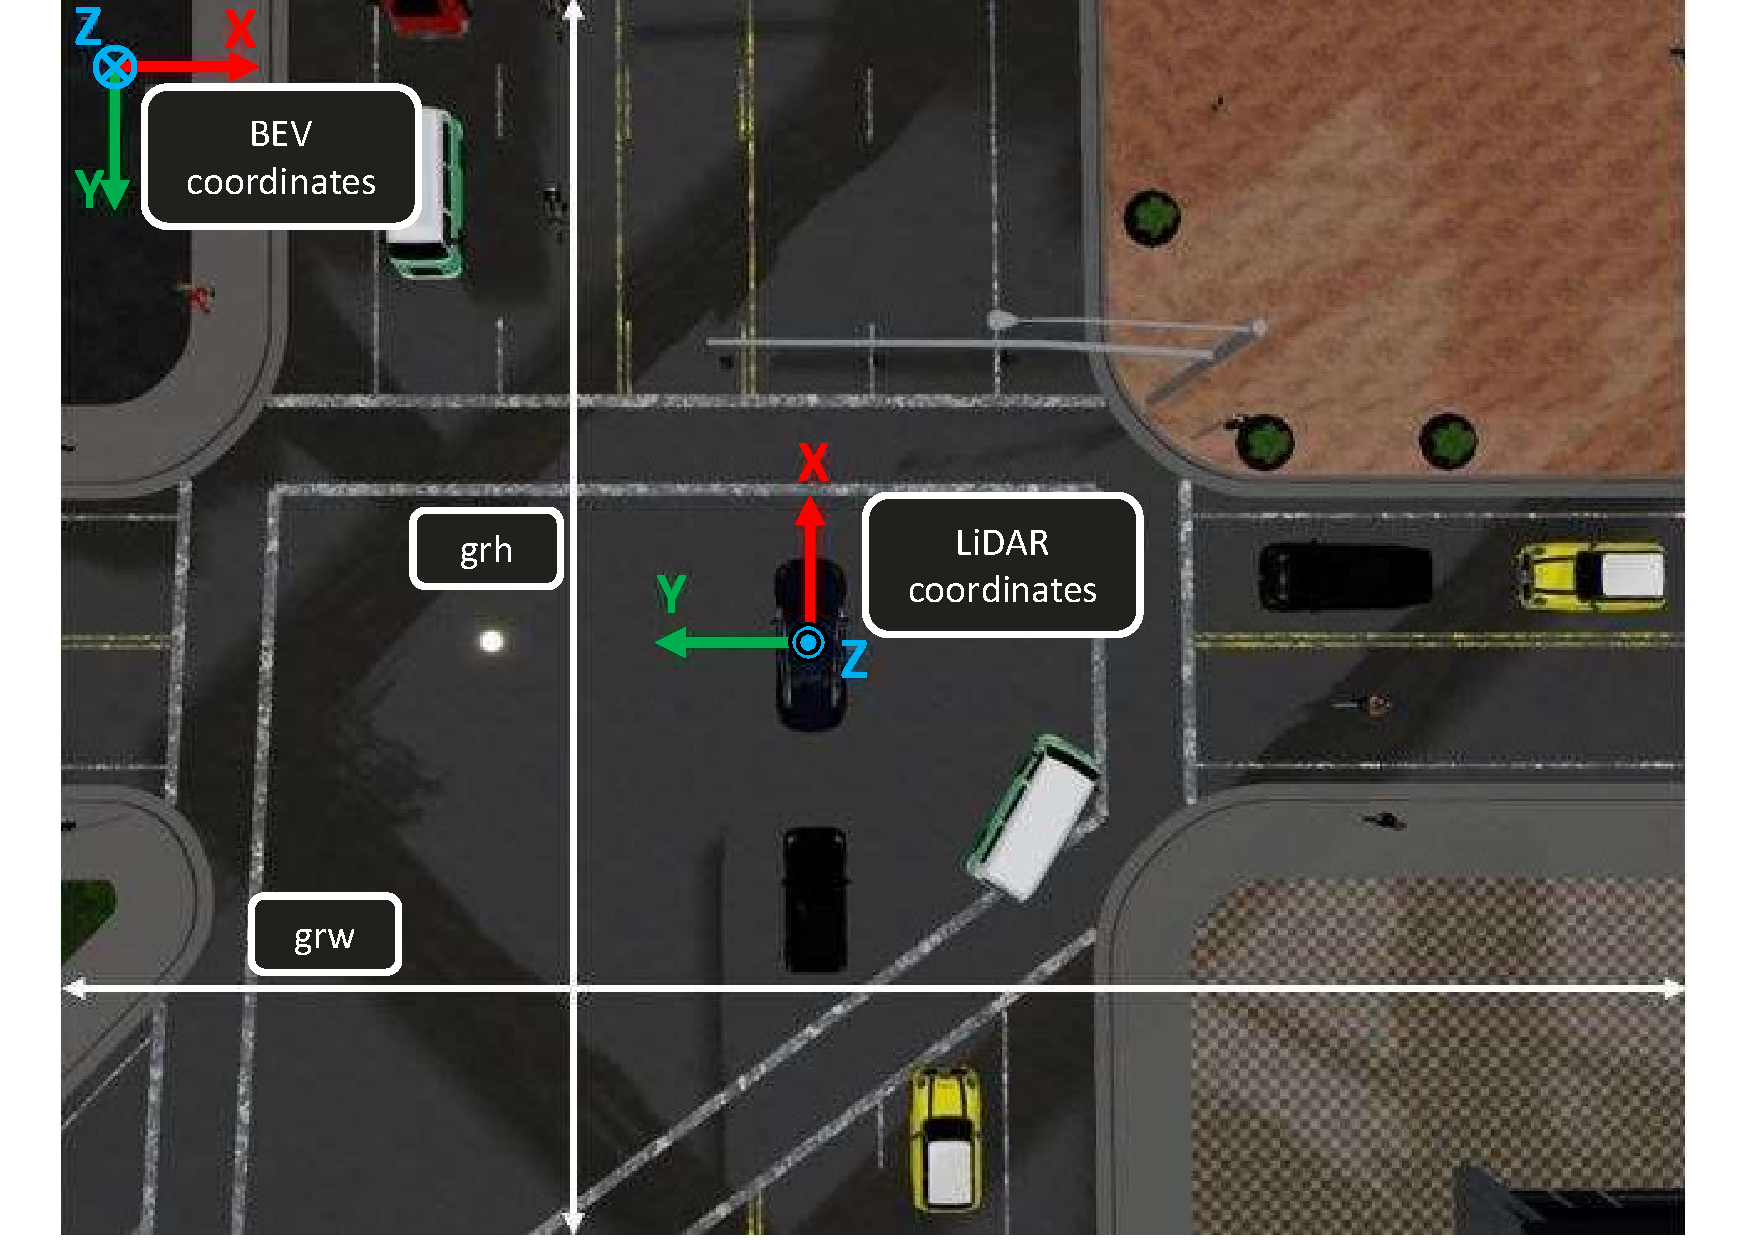
\includegraphics[width=0.42\textwidth]{chapter_4_SmartMOT/ITSC_2020_coordinates_conversion.pdf}
	\caption{LiDAR to BEV coordinates transformation illustrated in the CARLA simulator}
	\label{fig:chapter_4_SmartMOT/ITSC_2020_coordinates_conversion}
\end{figure}

\section{SmartMOT}
\label{sec:4_smartmot}

In order to solve the problem of monitoring the relevant objects in an efficient way, we propose SmartMOT \cite{gomez2021smartmot}, a simple-yet-accurate combination of traditional techniques such as the Kalman Filter (KF) \cite{kalman1960new} and Hungarian algorithm (HA) \cite{kuhn1955hungarian} for state estimation and data association respectively to solve the tracking-by-detection paradigm. Moreover, as mentioned in Section \ref{sec:4_introduction}, the core interest of SmartMOT is the incorporation of HD map semantic, geometric and topological information, in addition to the ego-vehicle status, so as to enhance the efficiency and reliability of the tracking system and subsequent predictions, as observed in Figure \ref{fig:chapter_4_SmartMOT/IV_2021}. 

The remaining content of this chapter summarizes the SmartMOT pipeline, being made up by: (1) 3D object detection module that returns the bounding boxes; (2) Monitored Area computation to filter non-relevant objects, \eg the VRUs that are inside the sidewalk far away the road or the vehicles that are located in a lane in which lane change is not allowed, (3) BEV Kalman filter that predicts the object state from the current frame and updates the object state based on the detected bounding boxes at current frame, (4) Hungarian algorithm which associates the current trackers with new detections, (5) Birth and Death memory that deals with the disappeared trajectories (unmatched trajectories exceeding ${age_{max}}$ frames) and the newly appeared trajectories (matched trajectories exceeding ${f_{min}}$ frames) and finally (6) \ac{CTRV} model which performs short-term physics-based motion prediction of the updated trackers information using both the linear and angular velocity information. As observed, except for the pre-trained object detector module (or ground-truth with the corresponding noise, if used), our \ac{MOT} system does not need any training and can be directly used for inference.

\begin{figure*}[thpb]
	\centering
	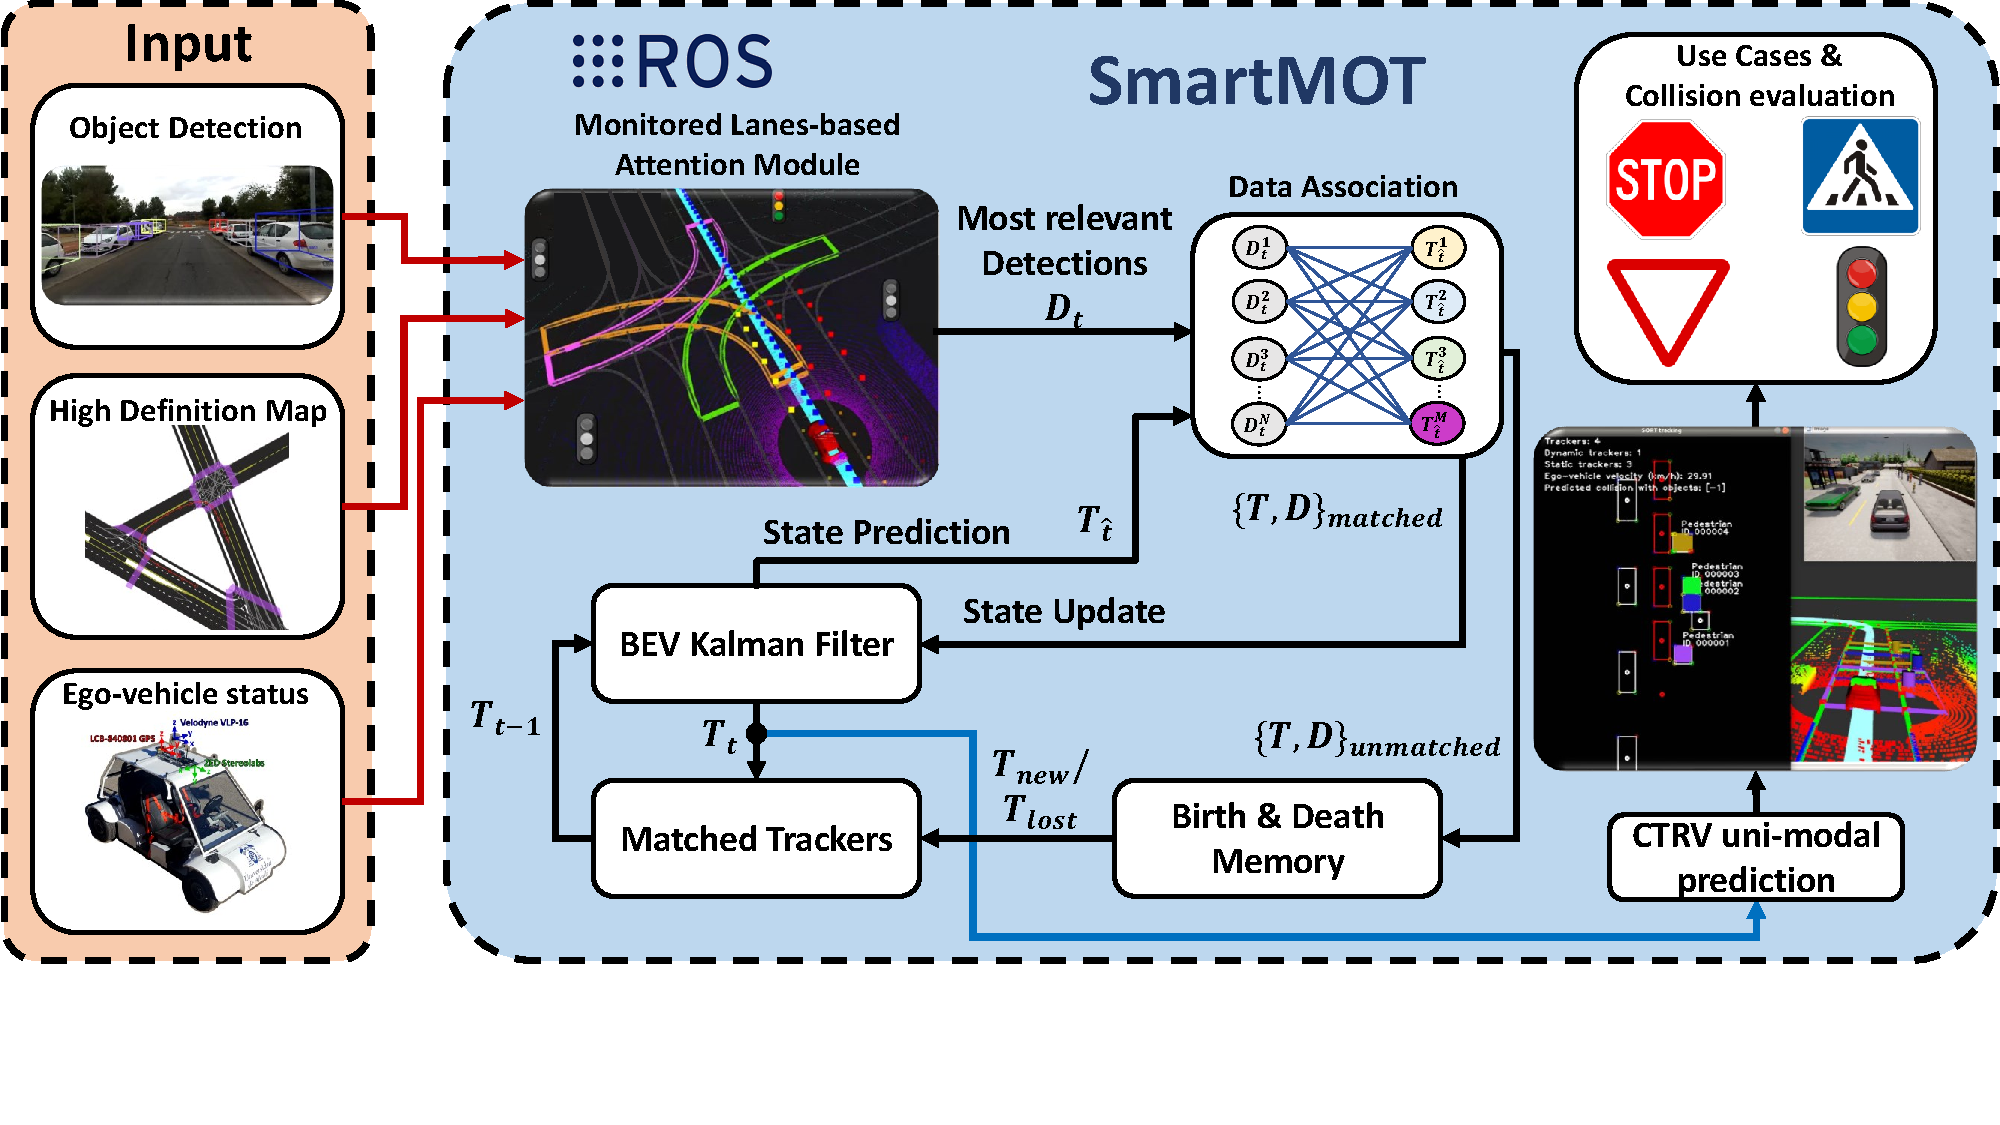
\includegraphics[width=\textwidth]{chapter_4_SmartMOT/IV_2021.pdf}
	\caption[SmartMOT pipeline]{$\textbf{SmartMOT pipeline}$: $\textbf{(1)}$ The object detection module, mapping layer and localization layer provide the 3D bounding boxes at frame \textit{t}, monitored lanes and ego-vehicle status data respectively; $\textbf{(2)}$ A Monitored Lanes-based Attention Module filters the non-relevant traffic participants and transforms the remaining into the \ac{BEV} image plane; $\textbf{(3)}$ A \ac{BEV} Kalman filter predicts the state of trajectories in frame \textit{t-1} to current frame \textit{\^{t}} throughout the prediction step; $\textbf{(4)}$ detections at frame \textit{t} and predicted trajectories at \textit{\^{t}} are matched using the Khun-Munkres (\aka Hungarian) algorithm; $\textbf{(5)}$ matched trajectories are updated based on their corresponding matched detections and every tracker is evaluated again based on its particular monitorized area, to obtain updated trajectories at frame \textit{{t}}; $\textbf{(6)}$ Unmatched trajectories and detections are used to delete disappeared trajectories or create new ones respectively; $\textbf{(7)}$ Updated trackers at frame \textit{{t}} are predicted using a CTRV model and then evaluated using the monitors module.}
	\label{fig:chapter_4_SmartMOT/IV_2021}
\end{figure*}

\subsection{3D Object Detection}

The first step our \ac{MOT} algorithm must carry out is to detect the obstacles in the environment around the ego-vehicle. As we will see in Chapter \ref{cha:experimental_results_and_applications}, in order to avoid perspective distortion, we make use of some well known 3D and 2D object detection approaches \cite{lang2019pointpillars, redmon2016you} to perform sensor fusion and retrieve the bounding boxes in the 3D space. Nevertheless, since this thesis do not focus on the object detection stage of the perception layer, some experiments are conducted assuming ground-truth detection including Gaussian noise in the \textit{x,y,z} to simulate real-world detections. Then, at a given frame \textit{t}, the detections provided by the object detection module are given in the following form:

\begin{equation}
	\label{eq:5_smartmot_detection}
	\textbf{D}_{t} =[\textbf{D}_{t}^{1},\textbf{D}_{t}^{2}, ...,\textbf{D}_{t}^{N}]
\end{equation}

Where \textit{N} is the number of detected 3D bounding boxes at a given frame and threshold. At this point, instead of using all the 3D information of the object \cite{chiu2021probabilistic, weng20203d}, we take its projection on the floor plane (\ac{BEV} information), to reduce the complexity and computational cost of the tracking stage, specially in those urban scenarios full of vehicles, based on the assumption that the height (\textit{z}) dimension is not as important as other coordinates (\textit{x}-axis, \textit{y}-axis) in a context of self-driving navigation. Detected 3D bounding boxes are referred to the LiDAR coordinate system. A grid is applied to establish a relation between real-world and image dimensions to discretize the possible positions of the detected bounding boxes and decrease the complexity and computational cost of the tracking module. This grid is featured by a rectangle, whose center is located at the LiDAR position on the vehicle, where $\textit{grw}$ and $\textit{grh}$ represent its width and height in LiDAR coordinates $\textit{m}$ (meters) respectively. Then, each detection in Equation \ref{eq:5_smartmot_detection_tuple} is represented as the tuple:

\begin{equation}
	\label{eq:5_smartmot_detection_tuple}
	\textbf{D}_{t}^{i} = [x_{m},y_{m},w_{m},l_{m},\theta,type,score]
\end{equation}

Where $\textit{$x_{m},y_{m}$}$ correspond to the object centroid in LiDAR coordinates ($\textit{m}$), $\textit{$w_{m}$}$ and $\textit{$l_{m}$}$ correspond to the width and length of the object respectively ($\textit{m}$), $\theta$ its orientation angle around the LiDAR Z-axis, object type and detection confidence. Figure \ref{fig:chapter_4_SmartMOT/ITSC_2020_coordinates_conversion} illustrates the transformation from the source coordinate system (LiDAR), measured in $\textit{m}$ and placed at the ego-vehicle, to the target coordinate system (BEV), measured in $\textit{px}$ (pixels) and placed on the top-left corner of the grid, which is the most common way to work with images in computer vision. In other words, we deal with the \ac{MOT} problem from the \ac{BEV} image perspective, in order to adapt \ac{MOT} algorithms originally designed for computer vision purposes. 

Equations \ref{eq:5_smartmot_rw_to_image_transform} and \ref{eq:5_smartmot_rw_to_image_apply_transform} show the transformation matrix between both coordinate systems, including both the rotation and the translation (\textit{$\frac{gw}{2}$} and \textit{$\frac{gh}{2}$}), where a $\textbf{LiDAR}_{point}=[x_{m},y_{m},z_{m},1]^{T}$ is given as the column vector in homogeneous coordinates.

\begin{equation}
	\label{eq:5_smartmot_rw_to_image_transform}
	\textbf{T} = \left[ \begin{array}{cccc}
		0  &  -1 &  0  &  \frac{grw}{2} \\
		-1 &  0  &  0  &  \frac{grh}{2} \\
		0  &  0  &  -1 &  0            \\
		0  &  0  &  0  &  1 \end{array} \right] 
\end{equation}

\begin{equation}
	\label{eq:5_smartmot_rw_to_image_apply_transform}
	\textbf{BEV}_{point} = \textbf{T} \cdot \textbf{LiDAR}_{point}
\end{equation}

At this point, each detection is represented by the tuple shown in Equation \ref{eq:5_smartmot_detection_tuple}, but now \textit{$x_{m},y_{m}$} represent the obstacle centroid in \ac{BEV} image perspective. Furthermore, the resolution of the \ac{BEV} image can be modified, in such a way the image width in pixels is given to the algorithm and the image height is calculated according to the aspect ratio of the real world with respect to the width of the image in pixels. Finally, to convert a point from real-word units ($\textit{m}$) to camera units ($\textit{px}$), we apply the corresponding scale factor to each coordinate:

\begin{equation}
	\label{conversion}
	\left[ \begin{array}{c}
		x_{px}  \\
		y_{pc} \end{array} \right] 
	=
	\left[ \begin{array}{cc}
		\frac{gpw}{grw} & 0  \\
		0 & \frac{gph}{grh} \end{array} \right]
	\left[ \begin{array}{c}
		x_{m}  \\
		y_{m} \end{array} \right] 
\end{equation}

However, it is very common to have different scales for $\textit{x}$ and $\textit{y}$-axis since it is more interesting to have a further view in the $\textit{x}$ LiDAR axis rather than a large side sweep in terms of $\textit{y}$ LiDAR axis. Considering this hypothesis, the right way to obtain the width and length of the \ac{BEV} LiDAR bounding box in $\textit{pixels}$ is to obtain the corners of the rotated bounding box in pixels and then compute the \textit{L2} (\aka Euclidean distance) among the corresponding corners to obtain the width and length in $\textit{pixels}$. Nevertheless, the object detector provides the rotation angle of the obstacle (featured as $\theta$) according to its own coordinate system and not around the ego-vehicle coordinate system. Regarding this constraint, to calculate the dimensions of the bounding box in pixels, three steps must be followed:

\[
c1_{m} = (x_{m}-\frac{l_{m}}{2},y_{m}-\frac{w_{m}}{2}) \]
\[
c2_{m} = (x_{m}-\frac{l_{m}}{2},y_{m}+\frac{w_{m}}{2}) \]
\[
c3_{m} = (x_{m}+\frac{l_{m}}{2},y_{m}-\frac{w_{m}}{2}) \]
\[
c4_{m} = (x_{m}+\frac{l_{m}}{2},y_{m}+\frac{w_{m}}{2}) \]

First, we assume a horizontal bounding box ($\theta$ = 0) at the BEV image coordinate system origin, where $\textit{c1}$ corresponds to the top-left corner ($\textit{c2}$, $\textit{c3}$ and $\textit{c4}$ are placed clockwise). Then, using the above equations for each corner, the Euclidean distance is applied between $\textit{c1}$ and $\textit{c2}$ to obtain the width in pixels, in the same way that the Euclidean distance is applied between $\textit{c1}$ and $\textit{c4}$ to obtain the length in pixels.

\begin{equation}
\label{widthpixels}
w_{px} = \sqrt{(c1_{px,x}-c2_{px,x})^2 + (c1_{px,y}-c2_{px,y})^2}
\end{equation}

\begin{equation}
\label{lengthpixels}
l_{px} = \sqrt{(c4_{px,x}-c2_{px,x})^2 + (c4_{px,y}-c2_{px,y})^2}
\end{equation}

Finally, the first four variables of the detection tuple shown in Equation \ref{eq:5_smartmot_detection_tuple} are converted into pixels, in such a way the tracking algorithm will monitor these bounding boxes in the BEV image by using the following tuple:

\begin{equation}
	\label{detpx}
	\textbf{D}_{t,i} = [x_{px},y_{px},w_{px},l_{px},\theta,type,score]
\end{equation}

\subsection{Monitored Lanes-based Attention Module}
\label{subsec:4_smartmot_mlam}

\acp{ADS} need to locate itself in the environment to know what is happening around in order to make decisions and execute a correct navigation like a human driver would. When we talk about localization, the first thing we need is a map where to be located and, particularly for vehicles, this is road map. Road maps used by current navigators, \eg Google Maps, are not valid for AV because of data type and the fact that they are not accurate enough to be used for autonomous driving. Here is where HD maps appear to solve this problem.

A HD map is usually a text file describing the real-world features related to the road map and its location within a 2D/3D space, and can do things that other sensors cannot \cite{wong2020mapping}: First, they have an \textit{infinite range} and, therefore, can \textit{see} even into occluded areas. Second, HD maps will never fail due to environmental conditions. Lastly, HD maps contain highly refined data. This information can be used by different modules of an AV, (including localization, vehicle control, path planning, perception and system management) drastically reducing the computational load and complexity in comparison to other more complex methods, providing robustness and reliability to the system.

\begin{figure}[] 
	\centering
	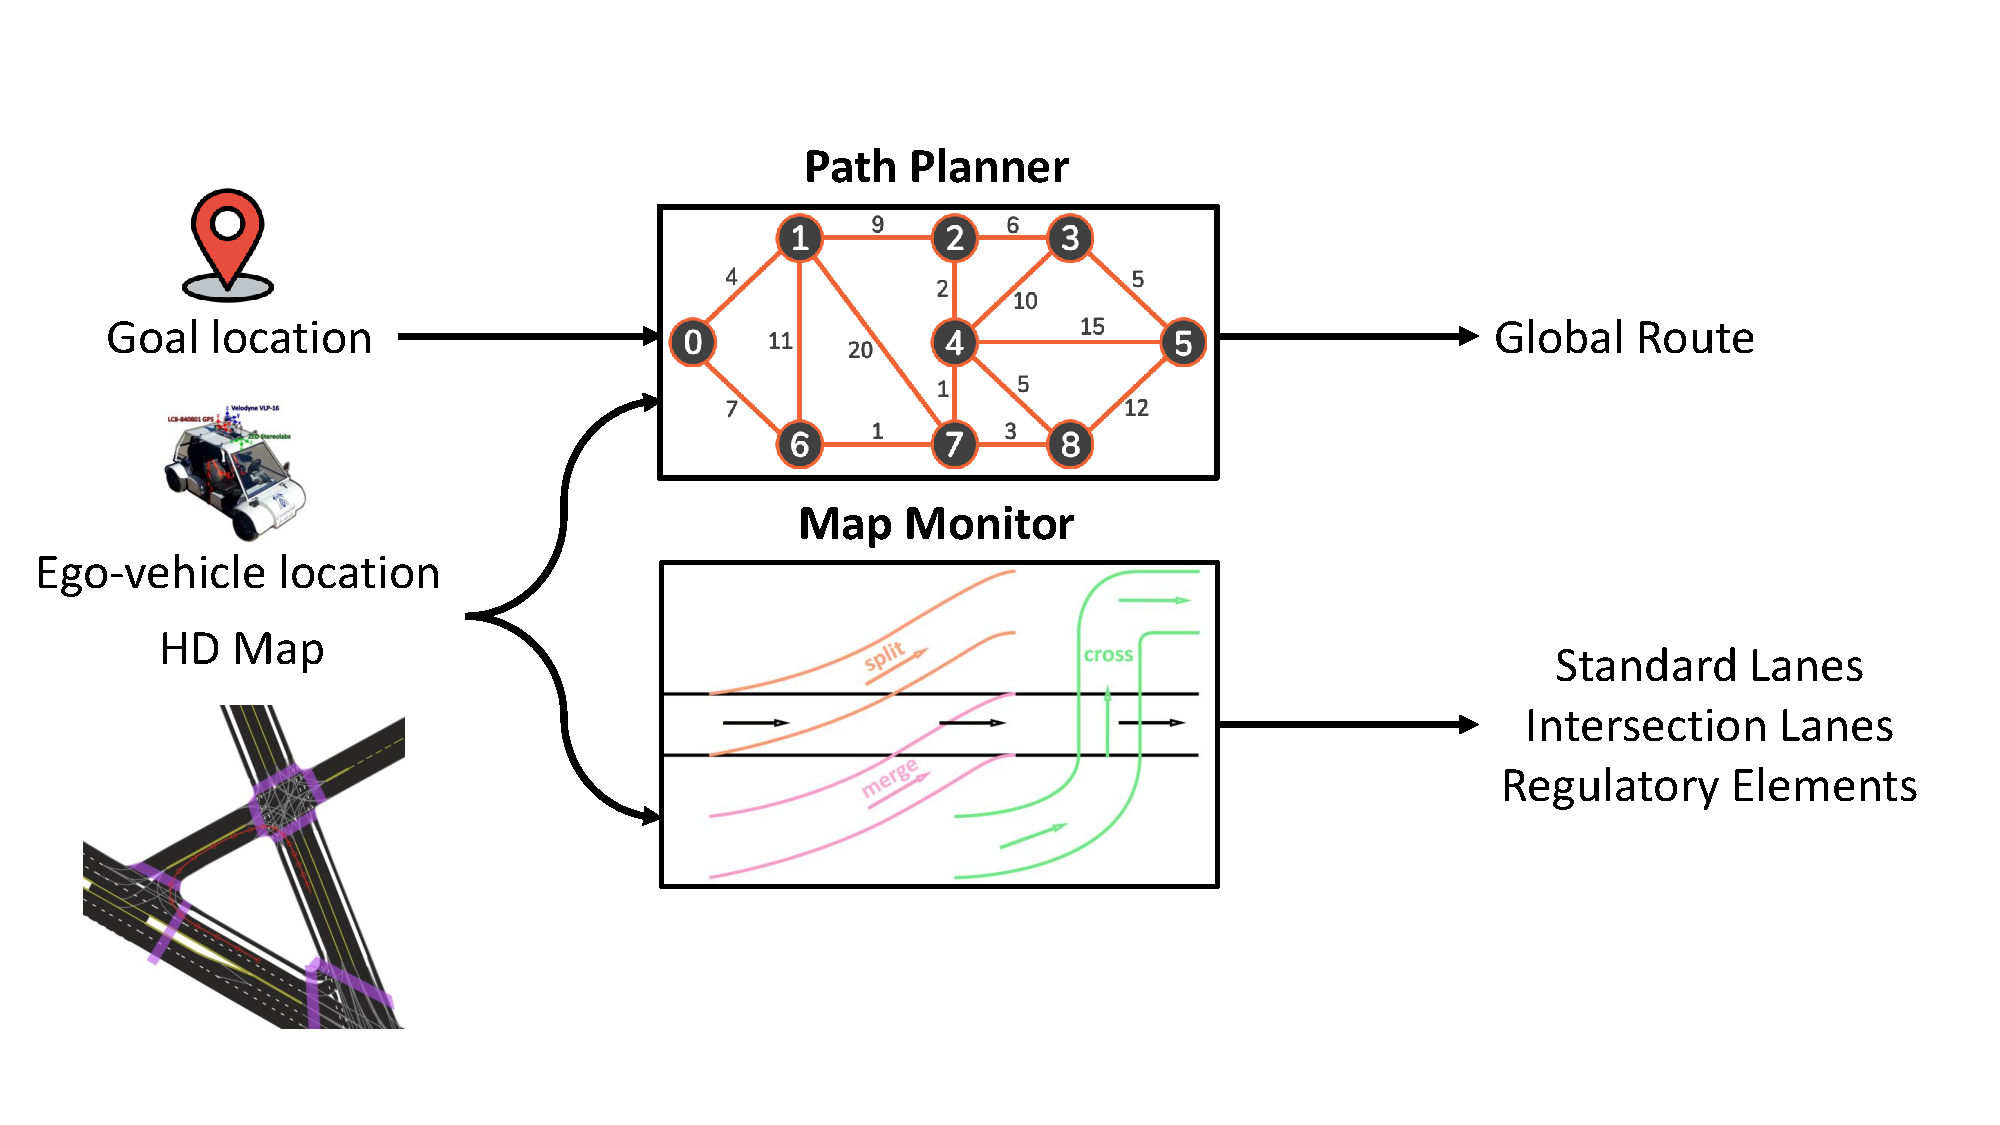
\includegraphics[width=0.8\textwidth]{chapter_4_SmartMOT/path_planner_map_monitor.pdf}
	\caption{Path Planning and Map Monitoring Outline}
	\label{fig:chapter_4_SmartMOT/path_planner_map_monitor}
\end{figure}

In terms of mapping information, we may distinguish three main categories:

\begin{itemize}
	\item Topological information provides the connectivity between geometry features. Particularly in the field of \ac{AD}, this is usually the network of roads. This kind of information can allow vehicles to traverse the most energy-efficient route, based on traffic speed, road grade or distance, as well as ensure that \acp{ADS} obey traffic regulation orders, such as one-way streets or the corresponding regulatory elements (pedestrian crossing, traffic light, stop signal, etc.).
	\item Geometric information provides the geometry or shape of other environmental features which can be static (permanent obstruction, such as buildings, bridges or tunnels), temporary (exist for only a limited amount of time, like traffic cones, parked vehicles or temporary road works) and dynamic features (moving people, objects or vehicles). Most of these features are incorporated by means of perception systems, specially in terms of dynamic features, in order to include that information in the HD map for successful motion planning and prediction.
	\item Semantic information returns the \textit{meaning} of aforementioned features, such as road speed limit, road classification, lane information or even the relational information among the different lanes, \ie how lanes work together, different types of lanes, where vehicles must stop and where vehicles can and cannot turn.
\end{itemize}

As illustrated, providing rich physical contextual information allows \acp{ADS} to make informed decisions in different driving scenarios. In our group, we particularly make use of the OpenDrive \cite{dupuis2010opendrive} HD map format, which has been mainly used for two different purposes, as shown in Figure \ref{fig:chapter_4_SmartMOT/path_planner_map_monitor}:

\begin{itemize}
	\item Global Path Planning, which uses a specific path planner which inputs are the HD map information and the ego-vehicle current location to retrieve an optimal (usually optimized based on the travelled distance) global route towards an specific goal.
	\item Map monitoring, responsible for monitoring the most relevant static and dynamic map elements around the ego-vehicle at each timestep, such as standard lanes (current, back), intersection lanes (merge, split and cross) and regulatory elements (e.g. give way, stop, pedestrian crossing, traffic light).
\end{itemize}

In particular, given a pre-defined global route, in this thesis we focus our interest on designing a map monitor module, responsible for retrieving the most relevant lanes around the ego-vehicle to enhance real-time perception and scene understanding requirements.

\subsubsection{Map Monitor}
\label{subsubsec:4_smartmot_mapmonitor}

In a similar way to humans that pay more attention to close obstacles, people walking towards them or upcoming turns rather than considering the presence of building or people far away, the perception layer of a self-driving car must be modelled to focus more on the salient regions of the scene \cite{sadeghian2019sophie} and the more relevant agents to predict the future behaviour of each traffic participant. In that sense, high-fidelity maps have been widely adopted to provide offline (also known as context) information to complement the online information provided by the sensor suite of the vehicle and its corresponding algorithms. Recent learning-based approaches \cite{hong2019rules} \cite{chai2019multipath} \cite{gao2020vectornet} \cite{casas2018intentnet}, which present the benefit of having probabilistic interpretations of different behaviour hypotheses, require to build a representation to encode the trajectory and map information. \cite{hong2019rules} assumes that detections around the vehicle are provided and focuses its work on behaviour prediction by encoding entity interactions with ConvNets. Intentnet \cite{casas2018intentnet} proposes to jointly detect traffic participants (mostly focused on vehicles) and predict their trajectories using raw LiDAR pointcloud and rendered HD map information. PRECOG \cite{rhinehart2019precog} aims to capture the future stochasiticity by flow-based generative models. Furthermore, MultiPath \cite{chai2019multipath} uses ConvNets as encoder and adopts pre-defined trajectory anchors to regress multiple possible future trajectories. 

As observed, recent \ac{DL}-based techniques use relatively complicated filters to predict, in an accurate way, the spatial features of the obstacles in the scene, increasing the complexity and computational cost of the system. On the other hand, traditional methods for behaviour prediction are rule based, where multiple behaviour hypothesis are generated based on constraints from the road maps. As stated above, road maps present some clear advantages over other perception sensors: They have "infinite range", so they can extract information even into occluded areas. Second, they do not fail under challenging environmental conditions, such as intense fog or rain. Third, recent HD maps contain highly refined data (in which many hours or days of human verification and preprocessing to reduce noise and uncertainty), quite useful to perform safe navigation. Then, HD maps can be an additional sensor that cannot fail unless the road infrastructure changes, providing meaningful, accurate and useful information in real-time operation.  

Regarding this, we design a Map Monitor in charge of monitoring the surrounding area of the vehicle. The inputs of the Map Monitor are the information provided by the Map Parser module (in charge of getting the information of the map from the HD map file and transform it into custom classes that can be used by other modules like Planning or Perception) and the waypoint route previously obtained by the path planner. The main goal of the Map Monitor is to only monitor the most relevant map elements around the ego-vehicle given the route provided by the global planner (or a new route if the local planer decides to recalculate the route). 

First, the path planner returns the route which is divided in segments separated by a given distance and calculates in which segment of the route the ego-vehicle is found, activating a flag in such a way the Map Monitor can start operating. Otherwise, in case the ego-vehicle cannot be located inside the route, the Map Monitor is deactivated. Secondly, a monitor callback is called periodically every time the ego-vehicle status (position, velocity, orientation, etc.) is received, as observed in Figure \ref{fig:chapter_4_SmartMOT/IV_2021}. This callback evaluates, if the Map Monitor module is active, calculates the monitored elements frontwards and backwards for a given distance which is proportional to the ego-vehicle velocity given a braking distance linear model that establishes a linear regression between two arrays of velocity and braking distance data. Nevertheless, we make use of a threshold distance to avoid not monitoring if the ego-vehicle is stopped. %We will detail the corresponding hyperparameters in Chapter \ref{sec:5_mot_and_euroncap}.

The monitored elements are:

\begin{itemize}
	\item \textbf{Standard Lanes}: Current, back and the corresponding left and right lanes. Current lane is monitored from current position to a dynamic distance depending on the velocity of the ego-vehicle. Back lane is monitored from current position to back a proportional distance of the dynamic current lane obtained distance. Left and right lanes are monitored the same distance that current and back only if the lane marking from the HD map data allows the lane change.
	\item \textbf{Intersection Lanes}: Other lanes that intersect the current monitored lane are checked. Intersection lanes can have different roles: split (1 lane splits into 2 or more), merge (2 or more lanes merge into 1) and cross (a lane crosses a part of the current lane). To calculate the intersection lanes, each lane of every junction (junctions are areas where more than 2 roads meet) in the current lane is evaluated. The polygon of each lane is calculated and evaluated if is inside the polygon of the current lane. It is important to consider that roundabouts are considered as a set of multiple junctions. 
	\item \textbf{Regulatory Elements}: The monitored elements are stops, giveaways, traffic lights, speed limits and crosswalks. The regulatory elements are only monitored for the next intersection affecting the route. 
\end{itemize}

An example of our map monitor module in the CARLA simulator \cite{dosovitskiy2017carla} using the ROS \cite{quigley2009ros} visualizator (R-VIZ) may be observed in Figure \ref{fig:chapter_4_SmartMOT/monitored_area_CARLA_ROS}:

\begin{figure}[!ht] 
	\centering
	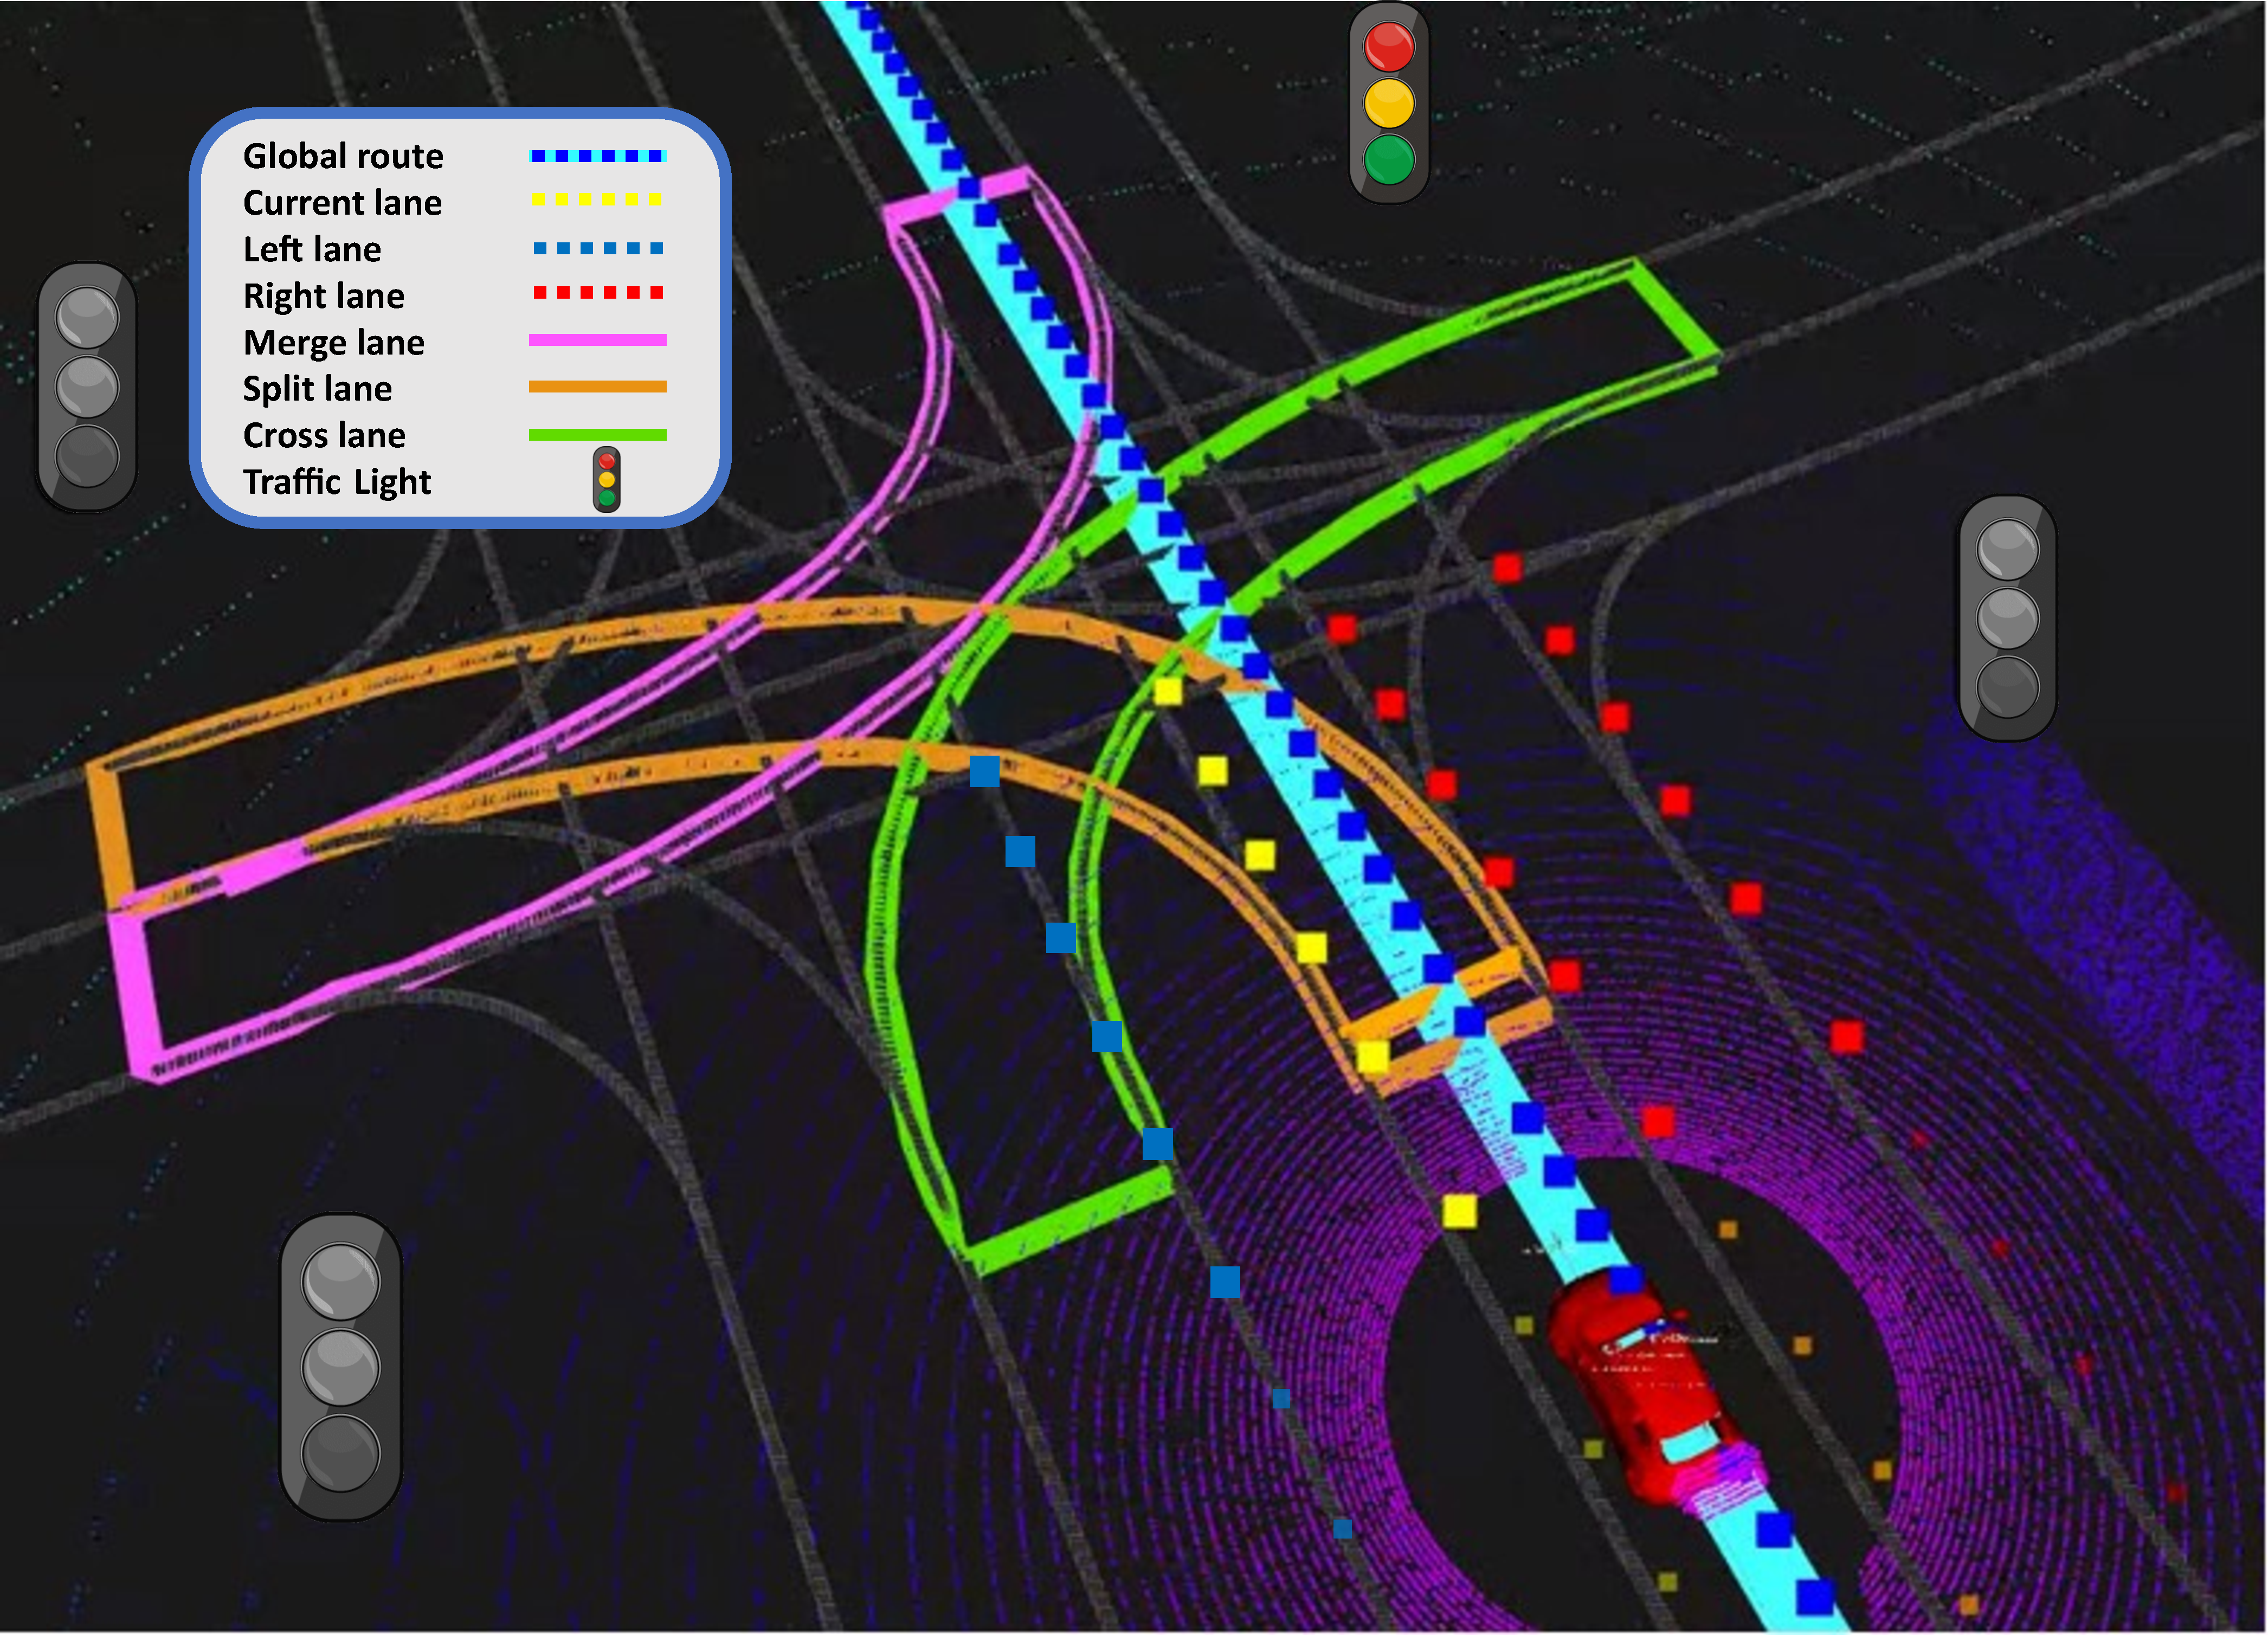
\includegraphics[width=0.8\textwidth]{chapter_4_SmartMOT/lane_types.pdf}
	\caption[Monitored area in the CARLA simulator using ROS visualizator (R-VIZ)]{Monitored area in the CARLA simulator using ROS visualizator (R-VIZ). It can be appreciated the visualization of the global route, standard lanes, intersection lanes and different traffic lights (regulatory elements). Note that the relevant traffic light is coloured while remaining ones are masked.}
	\label{fig:chapter_4_SmartMOT/monitored_area_CARLA_ROS}
\end{figure}

As illustrated in Figure \ref{fig:chapter_4_SmartMOT/IV_2021}, once the object detections have been provided and the monitored area has been computed, the Monitored Lanes-based Attention Module helps us to increase the efficiency and robustness of the system to avoid tracking and predicting all obstacles in the environment, which would escalate the computational cost especially in arbitrarily complex urban scenario. This attention module is not focused on \ac{DL} since the main purpose is to filter non-relevant obstacles in an efficient and interpretable way, such as agents driving way in opposite direction lanes, parked vehicles or pedestrians who are chatting on the sidewalk. The filtering process carried out by our Monitored Lanes-based Attention Module is summarized as follows:

\begin{algorithm}[H]
	\SetAlgoLined
	\KwData{point, polygon}
	\KwResult{isInside}
	crossings $\leftarrow$ 0\;
	\For{i from 0 to (polygon.length - 1)}{
		vertex1 $\leftarrow$ polygon[i]\;
		vertex2 $\leftarrow$ polygon[(i + 1) mod polygon.length]\;
		\If{(point.y > min(vertex1.y, vertex2.y)) \textbf{and} (point.y $\leq$ max(vertex1.y, vertex2.y))}{
			\If{point.x $\leq$ max(vertex1.x, vertex2.x)}{
				\If{vertex1.y $\neq$ vertex2.y}{
					xIntersection $\leftarrow$ (point.y - vertex1.y) * (vertex2.x - vertex1.x) / (vertex2.y - vertex1.y) + vertex1.x\;
					\If{vertex1.x == vertex2.x \textbf{or} point.x $\leq$ xIntersection}{
						crossings $\leftarrow$ crossings + 1\;
					}
				}
			}
		}
	}
	isInside $\leftarrow$ (crossings \% 2 == 1)\;
	\KwRet{isInside}\;
	\caption{Jordan's Curve theorem to determine if a point is inside a polygon}
	\label{alg:4_jordan_curve_theorem}
\end{algorithm}

\begin{enumerate}
	\item First, we determine the lanes of interested around the vehicle, till a given threshold. The minimum information will be the current front and back lane information (mandatory for the Adaptive Cruise Control and Unexpected Pedestrian use cases), as well as left and right lane information if lane change is available considering the presence of a discontinuous line. Moreover, if an intersection is near the ego-vehicle, other lanes of interest such as merging, splits and intersections are considered, which are specially useful in urban scenarios when the vehicle faces a roundabout or other vehicles incorporation in an intersection.
	\item In order to consider an agent as relevant, we study the presence of this agent in our monitored lanes in an elegant and efficient way. The main idea is to find the polygon segment (two nodes on the left, same on the right) closest to the agent. To do that, we iteratively compute the \textit{L2} distance between the agent position (transformed into global (\aka map) coordinates) and the left way nodes (starting from the beginning) of a certain lane. Note that it is irrelevant to take either the left or right lane in terms of observing if the detection is inside a polygon made up by four nodes of the lane, such as there exists the same number of nodes for both ways. For example, in the case of an agent located in front of the vehicle, the distance will decrease since the subsequent left way nodes are closer to the agent. 
	\item Once the new calculated distance is greater than the previous value, that means the closest segment with nodes \textit{$N_0$} and \textit{$N_1$} are found. Taking the same lane indexes in the right way, we obtain a 4-side polygon in which the detection is evaluated using the Jordan curve theorem \cite{tverberg1980proof}, as depicted in Algorithm \ref{alg:4_jordan_curve_theorem}. In this theorem, the input parameters are a point and a polygon, where, by means of a simple-yet-accurate ray casting algorithm, a loop is used to iterate over the polygon vertices and performs the necessary checks to determine the number of crossings. The Jordan's Curve Theorem states that a point is inside a polygon if the number of crossings from an arbitrary direction is odd. Consequently, in our particular case, if the object detection lies outside the closest polygon segment, the traffic participant is considered as non-relevant.
	\item Nevertheless, despite this proposal is coherent for non-holonomic obstacles with more constrained behaviours like cars, vans or trucks, the behaviour of Vulnerable Road Users (VRUs), such as pedestrians or cyclists, is usually difficult to predict. Hence, we widen the closest segment area a certain threshold \textit{L} to the sidewalk so as to track the closest VRUs to the road.
\end{enumerate}

\subsection{BEV Kalman Filter: State Prediction}
\label{subsec:4_smartmot_state_prediction}

Once we have obtained the most relevant \ac{BEV} detections of the environment, a \ac{BEV} Kalman Filter is used to track the objects. To predict the state of object trajectories from the previous frames to the current frame, we approximate objects inter-frame displacement using a constant velocity model which is independent of other objects in the scene and of the LiDAR motion. Regarding this, the estimation of the measured variables in the following frame are:

\[
x_{px}(\hat{t})=x_{px}(t)+v_{x} \:\:\:\:\:\: ; \:\:\:\:\:\: y_{px}(\hat{t})=y_{px}(t)+v_{y}\]
%\[
%y_{px}(\hat{t})=y_{px}(t)+v_{y} \]
\[
s(\hat{t})=s(t)+v_{s} \:\:\:\:\:\: ; \:\:\:\:\:\: 
\theta(\hat{t})=\theta(t)+v_{\theta}\]
%\[
%\theta(\hat{t})=\theta(t)+v_{\theta} \]

Since we formulate the tracking problem over the \ac{BEV} plane, we remove all variables related to the third dimension of the object, such as its $\textit{z}$ coordinate of the 3D bounding box centroid, its associated velocity and the height of the obstacle. On the other hand, since our tracking-by-detection algorithm is inspired by the well-established SORT (Single Online and Real Time) \cite{bewley2016simple} tracking model, originally proposed to track pedestrians using videos as input, some additional variables are included in the object state, such as the aspect ratio and the scale of the bounding box. The aspect ratio can be defined as the relation between the width and the length of the obstacle. Likewise, the scale represents the area of the target bounding box. Then, the state of each object tracker (usually referred as trajectory tracker in the literature) can be expressed as:

\begin{equation}
	\label{state}
	\textbf{T}_{t}^{j} = [x_{px},y_{px},s,r,\theta,x_{px}^{'},y_{px}^{'},s^{'},\theta^{'}]
\end{equation}

Note that the angular velocity $\theta^{'}$ is used in the state space to improve the prediction of the obstacle in later frames. Furthermore, as shown in \cite{bewley2016simple}, the aspect ratio of the bounding box is considered to be constant. As observed in Figure \ref{fig:chapter_4_SmartMOT/IV_2021}, at every frame \textit{t}, a tuple $\textbf{T}_{t}=[\textbf{T}_{t}^{1},\textbf{T}_{t}^{2}, ...,\textbf{T}_{t}^{M}]$ is returned by the data association module, where each element correspond to an association between a detection and a tracker. Note that $M$ represents the current number of trackers. Then, based on these associations between trackers of the previous frame and current detections, and assuming a Kalman Filter of first order (constant velocity model), the tuple $\textbf{T}_{\hat{t}}$ is calculated, where each element corresponds to the predicted trajectory ($\textbf{T}_{\hat{t}}^{j}$) in the current frame $\textit{t}$ expressed as:

\begin{equation}
	\label{est}
	\textbf{T}_{\hat{t}}^{j} = [x_{px}(\hat{t}),y_{px}(\hat{t}),s(\hat{t}),r,\theta(\hat{t}),x_{px}^{'},y_{px}^{'},s^{'},\theta^{'}]
\end{equation}

This tuple of predicted trajectories based on the previous frame associations, in addition to the current frame detections, represents the inputs to the data association algorithm at frame $t$.

\subsection{Data association}

In order to associate the detections $\textbf{D}_{t}$ and the trackers information after the Kalman Filter state prediction $\textbf{T}_{\hat{t}}$, the Hungarian algorithm is applied. The resulting affinity matrix presents $N$ rows (number of detections at frame $t$) and $M$ columns, which correspond to the number of predicted trajectories based on the information of frame $t-1$. Each element of the matrix corresponds to the Intersection over Union (IoU) in the \ac{BEV} plane between every pair of predicted trajectory and detection. Then, following the principles stated in Algorithm \ref{alg:3_ha}, we solve the bipartite graph matching problem, rejecting the matching if the BEV-IoU metric is lower than a given hyperparameter $IoU_{th}$, giving rise to a set of matched detections ($\textbf{D}_{matched}$) and predicted trackers ($\textbf{T}_{matched}$) with the same length $H$ (the number of matches), as well as a set of unmatched detections ($\textbf{D}_{unmatched}$), where $P = N - H$ is the number of unmatched detections, and a set of unmatched trajectories ($\textbf{T}_{unmatched}$), where $Q = M - H$ is the number of unmatched detections.

\subsection{BEV Kalman Filter - Object State Update}

As observed in Figure \ref{fig:chapter_4_SmartMOT/IV_2021}, once we have the corresponding sets of matched detections and trajectories, based on the Kalman Filter prediction-update cycle, we update the state space of each trajectory based on its corresponding matched detection. To do that, we use the weighted average between the matched detection values and the state space of the trajectory tracker, according to \cite{kalman1960new}. 

On the other hand, in the same way that \cite{weng20203d}, we appreciate that this state update step does not work properly for obstacle orientation. The reason is simple: Unless the object detector is based on sensor fusion and vision information is included, the object detector cannot distinguish if the obstacle is rotated 0 or $\pi$, $\frac{\pi}{2}$ and $\frac{3\pi}{2}$, and so on, around its \textit{z}-axis. That is, the orientation may differ by $\pi$ in two consecutive frames. Then, if no orientation correction is applied, the Kalman Filter associated to the tracker can get easily confused, since it tries to adapts itself to the new orientation value rotating the object by $\pi$ in following frames, giving rise to a low BEV-IoU between new detections and predicted trajectories. However, regarding the assumption that obstacles must move smoothly and its orientation cannot be modified by $\pi$ in one frame (0.02 s assuming a frequency of 10 Hz), when this happens the orientation of the corresponding matched detection or matched tracker can be considered wrong. To solve this problem, the detection module only considers angle from 0 to $\pi$ (that is, if an angle exceeds $\pi$, it is substracted to the provided angle). Moreover, if the difference of orientation between a given matched detection and its corresponding matched trajectory is greater than $\frac{\pi}{2}$, as stated before, either the orientation of the detection or the orientation of the tracker is wrong. Finally, we add $\pi$ to the orientation of the tracker with the aim to be consistent with the matched detection. 

\subsection{Deletion and Creation of Track Identities}

When obstacles leave and enter the aforementioned monitored lanes, unique identities must be destroyed or created accordingly. In most tracking algorithms it is known as the Birth and Death Memory, which is based on the set of unmatched trackers and detections provided by the data association algorithm, where the unmatched trackers represent potential objects leaving the monitored area, in the same way that unmatched detections represent potential objects entering in the area of interest. 

In order to avoid tracking of false positives or non-relevant obstacles, a new tracker is not created until the unmatched detection has been continuously detected in the next $f_{min}$ frames. Then, the tracker is initialized with the features of the detected bounding box, and the associated velocities set to zero. Note that, as stated in \cite{bewley2016simple}, since the velocity associated to the measured variables is unobserved at this moment (i.e., tracker initialization), the covariance initializes the value of the velocities (in the present work, velocity of the $x_{px},y_{px}$ centroid, scale $s$ and rotation angle $\theta$) with large values, reflecting their uncertainty. 

To avoid removing true positives trajectories from the scene, they are not terminated unless they are not detected during consecutive $a_{max}$ frames. This assumption prevents an unbounded growth in the number of localisation errors and trackers due to predictions over long duration where the object detector does not provide any correction. Note that since this work does not consider object re-identification for simplicity, an object should leaves the scene and then reappers, according to the SORT algorithm, if it is initialized with a new tracker under a new identity. As shown in Figure \ref{fig:chapter_4_SmartMOT/IV_2021}, the inputs to the Matched Trackers module are the updated matched trajectories from the BEV Kalman Filter and a set of created and deleted trackers, which jointly represent the input trajectories for the prediction step in the following frame.

\subsection{CTRV prediction}
\label{subsec:4_smartmot_ctrv_prediction}

The last stage of our SmartMOT pipeline is a physics-based \ac{MP} model to predict the future behaviour of the agents in the short-term. In particular, we make use of the previously studied \ac{CTRV} model. Once the tracker information (position, velocity and orientation) has been retrieved in real-world coordinates (instead of \ac{BEV} image coordinates), we are able to differentiate between static and dynamic agents. Then, given the ego-vehicle status and dynamic agents short-term prediction, we are able to analyze the risk of collision or to carry out the state of the current behaviour (Adaptive Cruise Control, Pedestrian Crossing, etc.) in such a way SmartMOT can send a signal to suddenly stop the car. Further experiments will be detailed in Chapter \ref{sec:5_mot_and_euroncap}. Figure \ref{fig:chapter_4_SmartMOT/filtering_process_example} illustrates an example of the filtering process, tracking-by-detection paradigm and \ac{CTRV} prediction.

\begin{figure}[] 
	\centering
	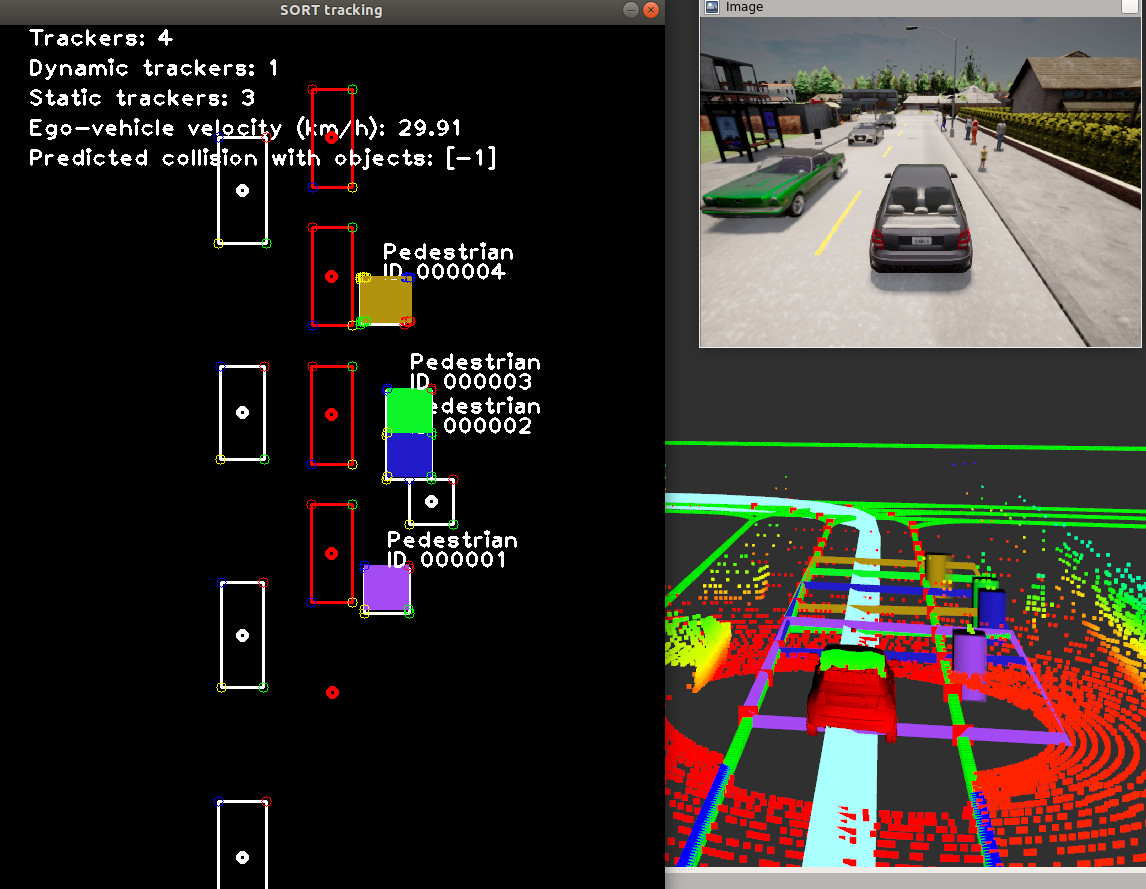
\includegraphics[width=0.8\textwidth]{chapter_4_SmartMOT/filtering_process_example.jpg}
	\caption{Vulnerable Road Users (VRUs) are considered on the sidewalk if the they are close enough to the closest segment of the corresponding centerline.}
	\label{fig:chapter_4_SmartMOT/filtering_process_example}
\end{figure} 

\section{Experimental results}
\label{sec:5_mot_and_euroncap}

As stated in Section \ref{sec:4_smartmot}, SmartMOT is a tracking pipeline that leverages HD map information to subsequently conduct a physics-base unimodal prediction. To validate this algorithm, we first validate the proposed tracking algorithm using the KITTI \ac{MOT} benchmark. Then, we conduct an interesting study of how integrating the monitored area can reduce the risk of collision and/or the impact velocity on the \ac{VRU}.

\subsection{Multi-Object Tracking performance}
\label{subsec:4_mot_results}

In order to evaluate our proposed \ac{MOT} system pipeline, we carry out the evaluation in the KITTI \ac{MOT} benchmark based on the method proposed by \cite{weng20203d}. The KITTI MOT benchmark is composed of 29 testing and 21 training/validation video sequences, where each sequence is provided with the corresponding RGB images (left and right camera of the stereo pair), LiDAR point cloud and the corresponding calibration file. Since KITTI does not provide any annotation (\ie, the groundtruth) for the testing split, we decided to evaluate our system in the training/validation split. Moreover, although KITTI distinguish among eight different classes for the object type, our work focus on the car subset, since it is the class that contains the most number of instances over the whole benchmark.

\subsubsection{Multi-Object Tracking metrics}
\label{subsubsec:4_mot_metrics}

Mainstream metrics applied to MOT systems are extracted from CLEAR MOT metrics \cite{bernardin2008evaluating}, such as MOTA (Multi-Object Tracking Accuracy), MOTP (Multi-Object Tracking Precision), ML/MT (Number of Mostly Lost/Tracked trajectories), IDS (Number of identity swutches), FRAG (Number of fragmentations generated by false negatives) and FN/FP (Number of false negatives/positives). These metrics provide a comprehensive assessment of tracking performance by considering aspects such as accuracy, precision, and overall performance:

\paragraph{MOTA (Multi-Object Tracking Accuracy)}
\label{par:4_MOTA}

The MOTA metric is commonly used to evaluate the performance of multi-object tracking algorithms. It measures the overall tracking accuracy by considering the false positives (FP), false negatives (FN), and identity switches (IDS) in the tracking results. The formula for calculating MOTA is given as:

\begin{equation}
	MOTA = 1 - \frac{{\text{{FN}} + \text{{FP}} + \text{{IDS}}}}{{\text{{GT}}}}
\end{equation}

where:

\begin{itemize}
	\item FN (False Negatives) represents the number of ground truth objects that were not correctly detected by the tracking algorithm.
	\item FP (False Positives) represents the number of false detections made by the tracking algorithm.
	\item IDS (Identity Switches) represents the number of times the algorithm incorrectly switches the identity of a tracked object.
	\item GT (Ground Truth) represents the total number of ground truth objects in the video sequence.
\end{itemize}

A higher MOTA value indicates better tracking accuracy, with a perfect tracking result yielding MOTA = 1.

\paragraph{MOTP (Multi-Object Tracking Precision)}
\label{par:4_MOTP}

The MOTP metric is used to assess the localization accuracy of a multi-object tracking algorithm. It measures the average precision of the tracked object positions by considering the distance between the predicted locations and their corresponding ground truth locations. The formula for calculating MOTP is given as:

\begin{equation}
	MOTP = \frac{{\sum_{{i=1}}^{{N}} d_i}}{{N}}
\end{equation}

where:
\begin{itemize}
	\item \(N\) represents the total number of matched object pairs between the predicted and ground truth locations.
	\item \(d_i\) represents the Euclidean distance between the predicted location and the ground truth location for the \(i\)-th matched object pair.
\end{itemize}

The MOTP metric ranges between 0 and 1, with a higher value indicating better localization accuracy. A perfect tracking result with exact object positions would yield MOTP = 1.

\paragraph{Integral metrics: AMOTA and AMOTP}
\label{par:4_integral_metrics}

Nevertheless, these metrics analyze the DAMOT system performance at a given threshold, not taking into account the confidence provided by the object detector and possibly misunderstanding the capability of the method. That means they do not take into account the full spectrum of precision and accuracy over different thresholds. Moreover, these traditional metrics evaluate the performance of the MOT system on the image plane (by projecting the detected 3D bounding box onto the image plane), which does not demonstrate the full strength of 3D DATMO. In that sense, AB3DMOT \cite{weng20203d} recently presented a 3D extension of the KITTI 2D MOT evaluation, known as KITTI-3DMOT, which focuses on the dimensions, orientation and centroid position of the 3D bounding box instead of the projection onto the image plane to evaluate the performance of the MOT system. Moreover, two new integral MOT metrics are introduced in order to solve the problem of evaluating the MOTA and MOTP of the system across all thresholds, known as AMOTA and AMOTP (Average MOTA and MOTP), as shown in Equation \ref{eq:5_amota}:

\begin{equation}
	\label{eq:5_amota}
	AMOTA = \frac{1}{L}\sum_{\{\frac{1}{L},\frac{2}{L},...,1\}}(1-\frac{FP+FN+IDS}{num_{gt}})
\end{equation}

Where $L$ is the number of different recall values. Note that IDS, FP and FN are modified according to the results of each threshold value. Likewise, AMOTP can be estimated by integrating MOTP across all recall values.

\subsubsection{MOT leaderboard}
\label{subsubsec:4_mot_leaderboard}

\begin{table}[h]
	\caption{Comparative of Multi-Object Tracking pipelines using the KITTI-3DMOT evaluation tool in the validation set (car class). We bold in \bf{black} the best results for each category}
	\label{table:4_MOT_pipelines_validation}
	\begin{center}
		\begin{tabular}{|c|c|c|c|c|c|}
			\hline
			Method & AMOTA &  AMOTP &  MOTA &  MOTP & IDs\\
			& (\%) & (\%) & (\%) & (\%) & \\
			\hline
			SmartMOT \cite{gomez2021smartmot} (tracking only) & 39.90 & \bf{79.31} & \bf{94.20} & 82.06 & 150 \\ 
			using PointPillars \cite{lang2019pointpillars} (Ours) & & & & & \\ \hline
			mmMOT \cite{zhang2019robust} & 33.08 & 72.45 & 74.07 & 78.16 & 10  \\ \hline
			FANTrack \cite{baser2019fantrack} & \bf{40.03} & 75.01 & 74.30 & 75.24 & 35 \\ \hline
			Monocular 3D \cite{weng2019monocular} & 31.37 & 64.29 & 62.38 & 68.26 & \bf{1} \\ \hline
		\end{tabular}
	\end{center}
\end{table}

We compare our proposed \ac{MOT} pipeline (PointPillars as 3D object detector \cite{lang2019pointpillars}, \ac{BEV} Kalman Filter, with the state space specified in Section \ref{sec:4_smartmot} as data estimator and Hungarian algorithm as data association algorithm) against modern open-sourced 3D MOT systems such as mmMOT \cite{zhang2019robust}, FANTrack \cite{baser2019fantrack} and Monocular3D \cite{weng2019monocular} using the proposed KITTI-3DMOT. Results are observed in Table \ref{table:5_MOT_pipelines_validation}, where we achieve results that are on-pair with other \ac{SOTA} tracking methods. Note that these results were obtained with default values of the hyperparameters in the tracking stage ($age_{max}$ = 1, $min_{hits}$ = 1, $IoU_{thr}$ = 0.1). For a deeper information of these hyperparameters, we refer the reader to the next subsection, where we conduct an ablation study to analyze the influence of maximum age or minimum threshold in the data association cost matrix to achieve the best tracking results.

% We evaluate our system using the KITTI-3DMOT evaluation tool proposed by \cite{weng20203d}, obtaining the results summarized in Table \ref{table:5_MOT_pipelines_validation}. In this table, we compare our numbers with the obtained by the representative state-of-the-art MOT system, AB3DMOT \cite{weng20203d}, with the following parameters: $IoU_{th}$ = 0.1 in the data association module, $f_{min}$ = 3 and $a_{max}$ = 2, and for two different object detectors: Pointrcnn \cite{shi2019pointrcnn} and Monocular 3D \cite{weng2019monocular}. Additionally, we include our previous proposal, which uses PointPillars \cite{lang2019pointpillars} as object detector, with an $IoU_{th}$ = 0.1 in the data association module, and $f_{min}$ = 1, $a_{max}$ = 3. Best results are coloured in black and the second best in blue. It can be appreciated the individual effect of using different 3D object detectors as well as using different hyperparameters in terms of tracking configuration. We get the best performance in three evaluated parameters, as well as the second best results in terms of MOTA, significantly improving our previous results for all parameters. Even though we do not overcome the results obtained by AB3DMOT using \cite{pointrcnn} as object detector, these are promising results since PointPillars configurations run at least twice faster with respect to remaining configurations, dealing with the real-time requirement in terms of autonomous driving.

\subsubsection{MOT ablation}
\label{subsubsec:4_mot_ablation}

Once we decide to implement a specific tracking-by-detection configuration, we carry out an ablation study that allows us to observe the performance in function of the tracking hyperparameters. These are:

\begin{itemize}
	\item \textbf{$age_{max}$: } Maximum number of frames for a tracker (Kalman Filter) to be associated again to a certain detection
	\item \textbf{$min_{hits}$: } Minimum number of consecutive frames in which a tentative tracker must be associated to a detection to be considered as an actual tracker
	\item \textbf{$IoU_{thr}$: } Threshold to match a predicted trajectory and a detection in the data association module
\end{itemize}

Table \ref{table:4_MOT_ablation} shows an ablation study by modifying these parameters. With a threshold $IoU_{thr}$ of 0.01 we get quite similar results in terms of MOTA and MOTP, decreasing by 36 $\%$ the number of identity switches (150 to 54). On the other hand, increasing the minimum number of hits allows us to reduce the identity switching noticeably, overcoming one of the main drawbacks associated to the motion metric proposed by SORT. Moreover, modifying the maximum age to consider a tracker has left the scene barely modifies the studied metrics. Finally, we bold in black the best values for each metric and in blue our final configuration ($age_{max}$ = 1, $min_{hits}$ = 3, $IoU_{thr}$ = 0.1) that achieves an impressive number of 2 identity switches and quite acceptable CLEAR and integral metrics, which are key as a preliminary stage to predict the short-term for each trajectory in the motion prediction stage.

\begin{table}[h]
	\caption{Ablation study of the final tracking stage configuration of SmartMOT using the KITTI-3DMOT evaluation tool in the validation set (car class). We bold the best results in \textbf{black} and the second best in \boldblue{blue} for each metric}
	\label{table:5_MOT_ablation}
	\begin{center}
		\begin{tabular}{|c|c|c|c|c|c|c|c|}
			\hline
			$age_{max}$ & $min_{hits}$ & $IoU_{thr}$ & AMOTA & AMOTP & MOTA & MOTP & IDs \\
			& & & (\%) & (\%) & (\%) & (\%) & \\
			\hline
			1 & 1 & 0.1 & \bf{39.90} & 79.31 & 94.20 & 82.06 & 150 \\
			\hline
			1 & 1 & 0.01 & 39.84 & 70.96 & 95.13 & 81.84 & 54 \\
			\hline
			1 & 1 & 0.25 & 39.37 & \bf{79.35} & 89.10 & 82.42 & 682 \\
			\hline
			\boldblue{1} & \boldblue{3} & \boldblue{0.1} & \boldblue{39.54} & \boldblue{71.24} & \boldblue{91.38} & \boldblue{83.23} & \boldblue{2} \\
			\hline
			1 & 5 & 0.1 & 39.26 & 71.36 & 88.84 & \bf{83.68} & 3 \\
			\hline
			2 & 1 & 0.1 & 39.49 & 79.24 & 94.91 & 81.48 & 154 \\
			\hline
			3 & 1 & 0.1 & 39.50 & 79.15 & \bf{95.16} & 81.15 & 152 \\
			\hline
		\end{tabular}
	\end{center}
\end{table}

Finally, our final system configuration is as following: We use PointPillars trained over 1,187,840 training steps using the KITTI MOT benchmark database, the BEV Kalman Filter formulated in the previous section, an $IoU_{th}$ = 0.1 as the threshold to associate a detection with a tracker the data association module, and $min_{hits}$ = 3, $age_{max}$ = 1 values for the birth and death module respectively. 

\subsubsection{Qualitative results in CARLA and our campus}
\label{subsubsubsec:4_mot_quali_carla_campus}

In this subsection we may appreciate some qualitative results both in simulation and in our real-world prototype using SmartMOT. One of the best advantages of CARLA is the possibility to create ad-hoc urban layouts by means of an OpenSCENARIO \cite{jullien2009openscenario} script definition where town, vehicles, climate conditions and also driving behaviours are defined, helpful to validate \ac{AD} algorithms (specially those focused on the perception layer) under different traffic and weather conditions. 

In terms of simulation, we reproduce a very common situation (as observed in the KITTI dataset) which is the $ego\_vehicle$ driving in narrow streets full of parked obstacles aside, evaluating its performance in night conditions. Despite this is probably the major disadvantage when using camera information (very poor performance in night conditions), we get impressive results in this situation, as illustrated in Figure \ref{fig:chapter_4_SmartMOT/MOT_CARLA}. This is pretty much coherent since LiDAR sensors are not passive sensors like cameras but they supply their own illumination source, which hits objects the reflected energy is detected and measured by the sensor in order to compute the distance to the object.

\begin{figure}[h]
	\centering
	\begin{subfigure}{0.24\textwidth}
		\captionsetup{justification=centering}
		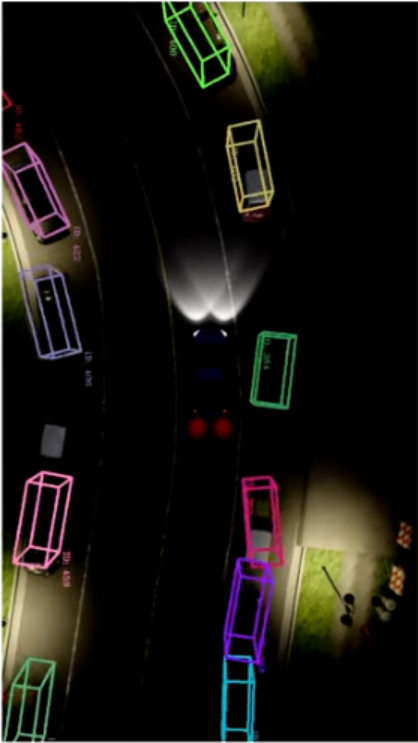
\includegraphics[width=4cm, height=6cm]{chapter_4_SmartMOT/qualitative/MOT_CARLA_1.PNG}
		\caption{}
	\end{subfigure}
	\hfill
	\begin{subfigure}{0.24\textwidth}
		\captionsetup{justification=centering}
		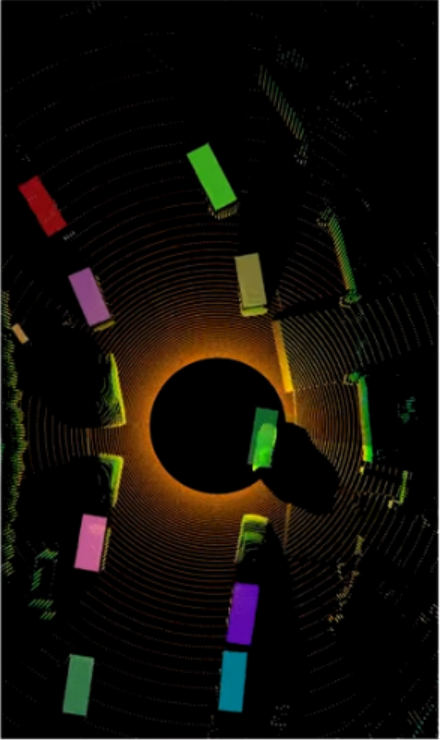
\includegraphics[width=4cm, height=6cm]{chapter_4_SmartMOT/qualitative/MOT_CARLA_2.PNG}
		\caption{}
	\end{subfigure}
	\hfill
	\begin{subfigure}{0.24\textwidth}
		\captionsetup{justification=centering}
		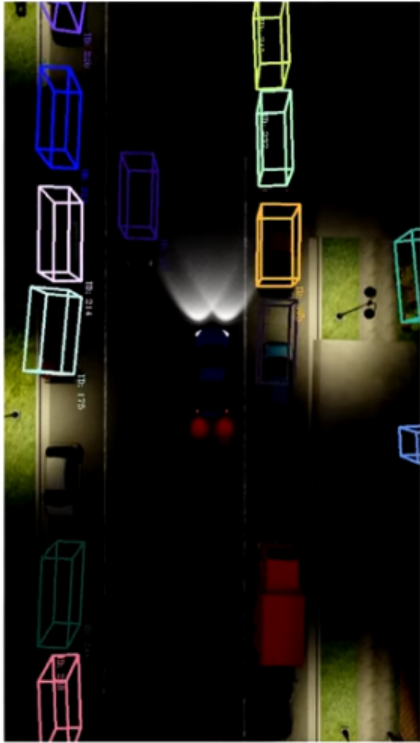
\includegraphics[width=4cm, height=6cm]{chapter_4_SmartMOT/qualitative/MOT_CARLA_3.PNG}
		\caption{}
	\end{subfigure}
	\hfill
	\begin{subfigure}{0.24\textwidth}
		\captionsetup{justification=centering}
		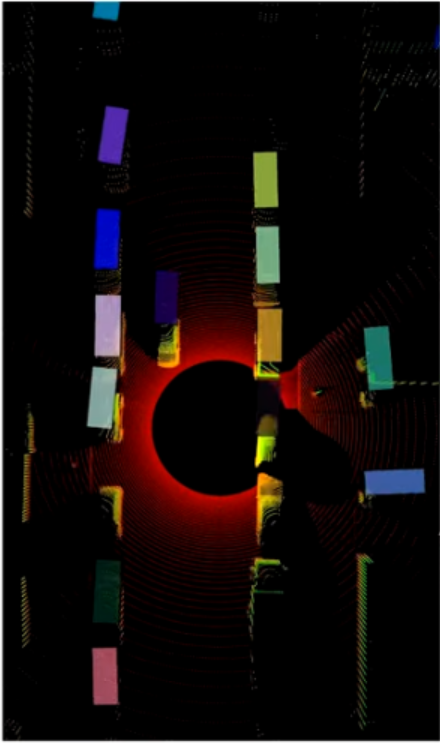
\includegraphics[width=4cm, height=6cm]{chapter_4_SmartMOT/qualitative/MOT_CARLA_4.PNG}
		\caption{}
	\end{subfigure}
	\caption[Detection and Tracking of Multiple Objects in the CARLA simulator]{Detection and Tracking of Multiple Objects in the parked aside vehicles at night traffic scenario considering a curved trajectory (a,b) and straight trajectory (c,d)}
	\label{fig:chapter_4_SmartMOT/MOT_CARLA}
\end{figure}

On the other hand, in terms of our real-world prototype, we focus on implementing a 360º real-time and power-efficient \ac{MOT} pipeline in an efficient way. Perception systems in autonomous driving must process a huge amount of information coming from at least one sensor in order to understand the environment. However, the physical space occupied by the processing units in the vehicle or their power consumption are metrics to be deeply analyzed, even more if these processing units will be integrated in an electric vehicle, where the state of the batteries is crucial. In that sense, the current approach is to use powerful but power-efficient \ac{AI} embedded systems as computation devices for autonomous machines, since they present a remarkable ratio between performance and power consumption in a reduced-size hardware. Regarding the advantage of using neural networks in GPU, these embedded systems present a powerful GPU unit as well as fast storages based on solid state disks and a large RAM memory size. At the time of writing this paper, the best ratio of performance vs power consumption and size is represented by the NVIDIA Jetson embedded computing boards. NVIDIA Jetson is the world's leading AI computing platform for GPU-accelerated parallel processing in mobile embedded systems. These kits allow to implement state-of-the-art frameworks and libraries to conduct accelerated computing, such as CUDA, cuDNN or TensorRT (Tensor RealTime). 

\begin{table}[h]
	\caption{Comparative of inference frequency between the NVIDIA Jetson AGX Xavier and our PC desktop (Intel Core i7-9700, 16GB RAM) with CUDA-based NVIDIA GeForce RTX 1080 Ti 11GB VRAM}
	\label{table:xavier_vs_computer_hz}
	\begin{center}
		\begin{tabular}{|c|c|c|c|c|c|}
			\hline
			Stage & Frequency AGX &  Frequency PC & Ratio \\
			& Xavier (Hz) & desktop (Hz) & \\
			\hline
			Detection & 7.3 & \bf{41.7} & 5.7x \\
			\hline
			Tracking & 15 & \bf{101.9} & 6.7x \\
			\hline
		\end{tabular}
	\end{center}
\end{table}

In this particular work we make use of the NVIDIA Jetson AGX Xavier, which is as far as we know one of the most powerful AI embedded system specially designed for autonomous machines. Table \ref{table:xavier_vs_computer_hz} shows a comparative between the embedded system and our PC frequency in the inference stage, where the detection (PointPillars) is reduced by almost 6 times and the tracking by almost 7 times. Nervertheless, although the detection and tracking frequencies are on the border to be considered real-time according to the requirements of the perception systems for autonomous machines, the embedded system consumes 30 W whilst only the 1080 Ti GPU consumes 250 W at full power respectively. Considering that the embedded system computation power is reduced by 6.2 times (average between the detection and tracking frequency ratios) but only the GPU (not considering the whole PC desktop) presents a power consumption 8.3 higher, makes the current NVIDIA Jetson AGX Xavier a better suitable option for large scale-deployment in the autonomous driving field rather than using desktop graphic cards. Distributing several sensor processing across multiple embedded systems for parallelization will result in lower power consumption than using conventional GPUs in future autonomous driving prototypes. Qualitative results of running our DAMOT pipeline in our own vehicle, equipped with a VLP-16 LiDAR instead of the HDL-64 shown in CARLA and KITTI, are illustrated in Figure \ref{fig:chapter_4_SmartMOT/MOT_campus}. It can be appreciated that although the obtained results are slightly worse than with the KITTI dataset (equipped with a HDL-64 sensor), we obtain quite promising results, validating the pipeline studied in this work both in terms of accuracy and real-time operation.

\begin{figure}[h]
	\centering
	\begin{subfigure}{0.43\textwidth}
		\captionsetup{justification=centering}
		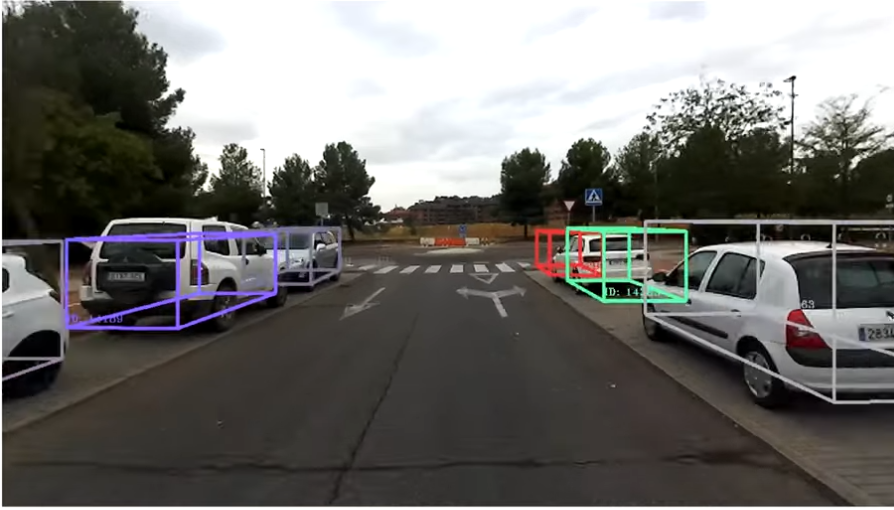
\includegraphics[width=\textwidth]{chapter_4_SmartMOT/qualitative/MOT_campus_1.PNG}
		\caption{}
	\end{subfigure}
	\hfill
	\begin{subfigure}{0.43\textwidth}
		\captionsetup{justification=centering}
		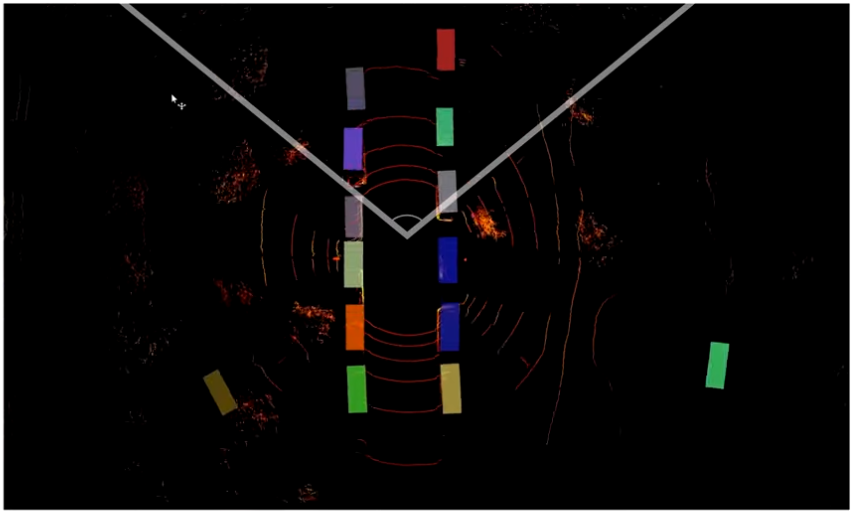
\includegraphics[width=\textwidth]{chapter_4_SmartMOT/qualitative/MOT_campus_2.PNG}
		\caption{}
	\end{subfigure}
	\hfill
	\begin{subfigure}{0.43\textwidth}
		\captionsetup{justification=centering}
		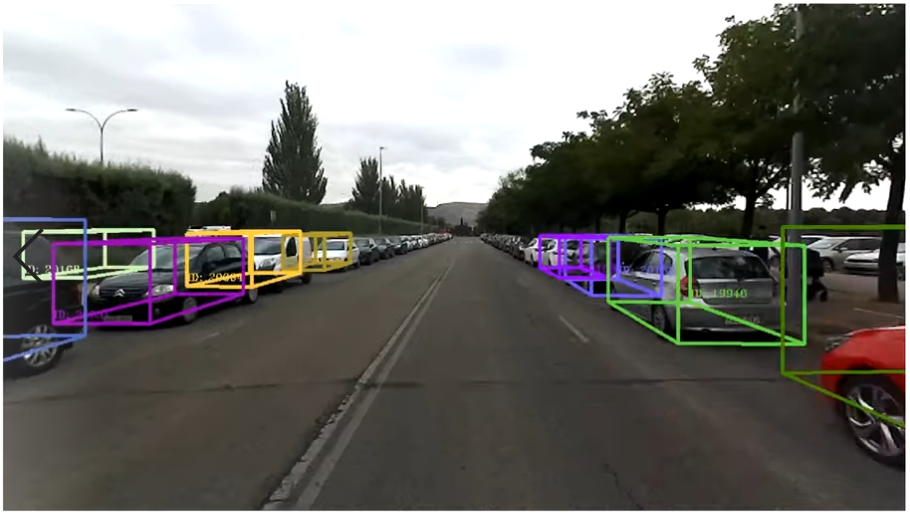
\includegraphics[width=\textwidth]{chapter_4_SmartMOT/qualitative/MOT_campus_3.PNG}
		\caption{}
	\end{subfigure}
	\hfill
	\begin{subfigure}{0.43\textwidth}
		\captionsetup{justification=centering}
		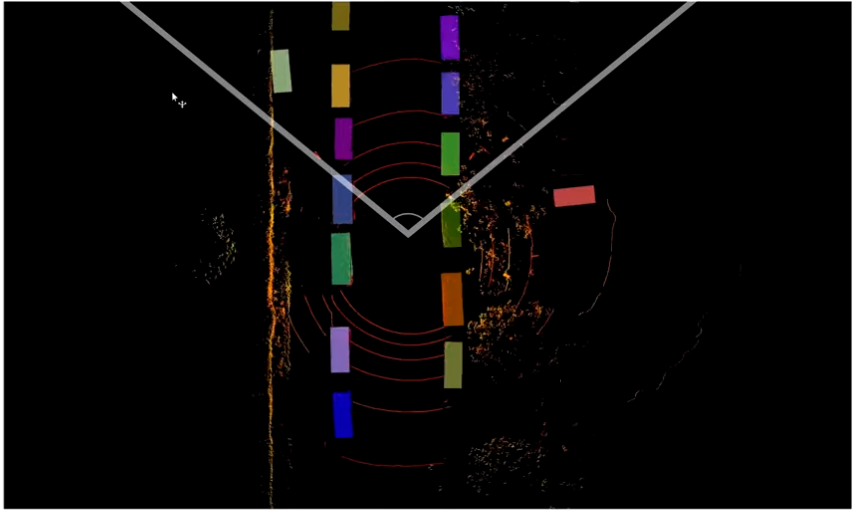
\includegraphics[width=\textwidth]{chapter_4_SmartMOT/qualitative/MOT_campus_4.PNG}
		\caption{}
	\end{subfigure}
	\caption{Detection and Tracking of Multiple Objects in our campus with our real-world vehicle}
	\label{fig:chapter_4_SmartMOT/MOT_campus}
\end{figure}

\subsection{EuroNCAP-based validation}
\label{subsec:4_euroncap}

A considerable amount of research works and studies, related to pedestrian detection and collision avoidance behavior are present in the literature, where the main objective is to validate the perception and control modules. Nevertheless, as stated before, we aim to demonstrate how incorporating HD map information helps the whole AD stack to anticipate faster the behaviour of the traffic participants in the corresponding traffic scenarios. Then, common metrics for all frameworks must be used to evaluate the whole architecture, where all modules are integrated. Regarding this, New Car Assessment Programs (NCAPs) protocols are introduced, evaluating the safety of vehicles for different traffic situations and Advanced Driver Assistance Systems, such as Child Occupant Protection (COP), Speed Assist Systems (SAS) or Autonomous Emergency Braking (AEB). Euro-NCAP \cite{article_EuroNCAP_2} is introduced in 1997, representing the widely most adopted performance assessment within the scope of the collaboration of European Union countries. China New Car Assessment Program (C-NCAP) \cite{article_CNCAP} is presented (2006) as a research and development benchmark for vehicle manufacturers in Asia, being most of its protocols based on Euro-NCAP. National Highway Transportation Safety Administration (NHTSA), funded in 1970 as an agency of the Department of Transportation of United States, published \cite{article_NHTSA} its guidance documents and regulations on vehicles equipped with ADAS. As observed, these programmes do not present specific protocols in order to evaluate AD stacks, presenting noticeable differences, such as different scenarios, parameters and evaluation metrics. 

Regarding this, in order to evaluate SmartMOT, we adopt the validation method proposed by \cite{gutierrez2021validation}, which proposes to generalize the \ac{VRU} v.10.0.3 protocol \cite{web_VRU_assessment_protocol}, representing a baseline to compare the performance of different pipelines for the particular situation (both in simulation and real-world) of an Unexpected Vulnerable Road User (VRU) jumping into the road during the navigation, where an Autonomous Emergency Braking (AEB) behaviour must be executed. 

\subsubsection{Implementation details of the EuroNCAP scenario}
\label{subsubsec:4_euroncap_implementation_details}

Figure \ref{fig:chapter_4_SmartMOT/CPNA_scenario} illustrates this traffic situation, in which the VRU (a pedestrian in this particular case) starts in the closest sidewalk to the vehicle in a perpendicular position to the vehicle orientation. Once the vehicle starts the navigation and the L2 distance between the ego-vehicle centroid and the VRU centroid is lower than a certain threshold \textit{d}, the VRU starts its path to unexpectedly cross the road in such a way the ego-vehicle must detect, track and forecast its future trajectory in order to avoid the collision or at least reduce the impact velocity as much as possible. Then, the protocol consists on reproducing the CPNA crash avoidance scenario, with a fixed VRU velocity (\(v_p\)) of 5 km/h and a variable ego-vehicle velocity that ranges from 10 km/h to 60 km/h. It is important to note that the threshold \textit{d} is not fixed, but it is ego-vehicle velocity dependent, that is, the pedestrian must start walking in such a way the impact point (\(P_I\)) (Figure \ref{fig:5_cpna_scenario}) is in the center of the lane for each particular velocity. 

\begin{figure}[h]
	\centering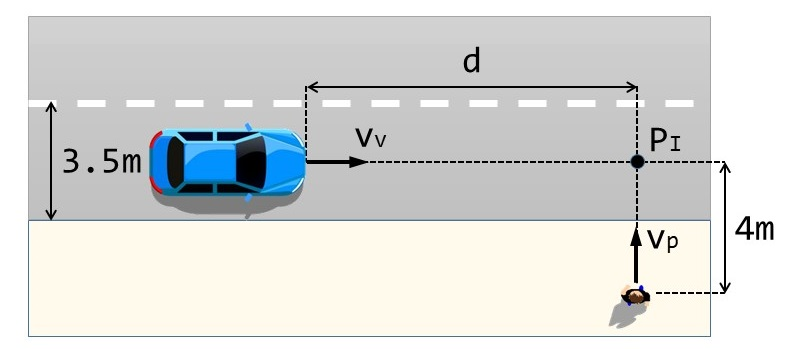
\includegraphics[width=0.4\textwidth]{chapter_4_SmartMOT/CPNA_scenario.jpg}
	\caption{Car to Pedestrian Nearside Adult (CPNA) scenario}	
	\label{fig:chapter_4_SmartMOT/CPNA_scenario}
\end{figure}

Regarding the evaluation metrics, a score for each test is calculated based on the velocity reduction of the vehicle, as following:

\begin{itemize}
	\item For a vehicle velocity \(v_v\) less than or equal to 40km/h:
	\begin{itemize}
		\item If the vehicle stops without collision, the highest score is achieved:
		\begin{equation}
			score_{test} = score_{max}
			\label{eq1}
		\end{equation}
		
		\item Otherwise, if the vehicle collides, its score is defined as follows:
		\begin{equation}
			score_{test} = \frac{v_{test}-v_{impact}}{v_{test}} \cdot score_{max}
			\label{eq2}
		\end{equation}
	\end{itemize}
	\item For \(v_v\) higher than 40km/h:
	\begin{itemize}
		\item If the vehicle is able to reduce its speed in at least 20 km/h, the highest score is achieve:
		\begin{equation}
			v_{impact} \leq v_{test} - 20 \to score_{test} = score_{max}
			\label{eq3}
		\end{equation}
		\item Otherwise, if the vehicle collides at a velocity greater than the velocity under test less a threshold of 20 km/h, no score is achieve:
		\begin{equation}
			v_{impact} > v_{test} - 20 \to score_{test} = 0
			\label{eq4}
		\end{equation}
	\end{itemize}
\end{itemize}

Finally, the final score of a particular pipeline is given by the arithmetic mean of the results obtained in each CPNA crash avoidance test for different weather conditions. For further details about the validation protocol, we refer the reader to \cite{gutierrez2021validation}.

\subsubsection{Experimental results in the EuroNCAP-based scenario}
\label{subsubsec:4_euroncap_experimental_results}

In this section we obtain some interesting both qualitative and quantitative results, evaluating our AD stack \cite{gomez2021train} in the CPNA crash avoidance scenario using two different perception layer strategies. On the one hand, we implement the perception module stated by \cite{gomez2020real} which tracks all objects in the environment regardless their topological information and considers a naive velocity dependent rectangular monitored area in front of the vehicle to determine the distance to the nearest object in the route as well as to predict the collision. On the other hand, we use SmartMOT to track and predict the future trajectories of only the most relevant obstacles around the vehicle, that is, those in which the human in manual driver should pay attention throughout the route, such as VRUs close to the road, vehicles in intersections and lanes where the lane change maneuver is allowed, etc. Qualitative results may be found in the following play list \href{https://cutt.ly/uk9ziaq}{SmartMOT} \footnote{SmartMOT: https://cutt.ly/uk9ziaq}, where the SmartMOT performance is illustrated. 

Regarding urban environment complexity, in order to validate a whole AD architecture the system must be tested in countless environments and scenarios, which would escalate the cost and development time exponentially with a physical approach. Considering this, the use of photo-realistic simulation (virtual development and validation testing) and an appropriate design of the driving scenarios are the current keys to build safe and robust AV. 

In our work we propose the use of CARLA (CAR Learning to Act) \cite{dosovitskiy2017carla} as the best open-source simulator to reach our goals, taking even more importance when analyzing the behaviours the vehicle can face in these complex traffic scenarios. One of the best advantages of CARLA is the possibility to create ad-hoc urban layouts, useful to validate the navigation architecture in challenging driving scenarios. This code can be downloaded from the ScenarioRunner repository, associated to the CARLA GitHub. The ScenarioRunner is a module that allows the user to define and execute traffic scenarios for the CARLA simulator. In the present case, we define several scenarios according to the CPNA crash avoidance traffic situation, modifying the velocity of the ego-vehicle and the presence of other traffic participants. All test were carried out in a PC desktop (Intel Core i7-9700k, 32GB RAM with CUDA-based NVIDIA GeForce RTX 2080 Ti 11GB VRAM), using the version 0.9.10.1 version of CARLA as well as the corresponding ROS Bridge, responsible of communicating the CARLA environment with our ROS-based architecture, and ScenarioRunner modules. In particular, we make use of the OpenScenario standard, supported by ScenarioRunner, where both the VRU and ego-vehicle features can be modified to accomplish the Euro-NCAP requirements. % Due to size constraint of this paper, we do not validate the performance of our architecture for different weather conditions but only in daytime conditions. 

\begin{figure}[h]
	\centering
	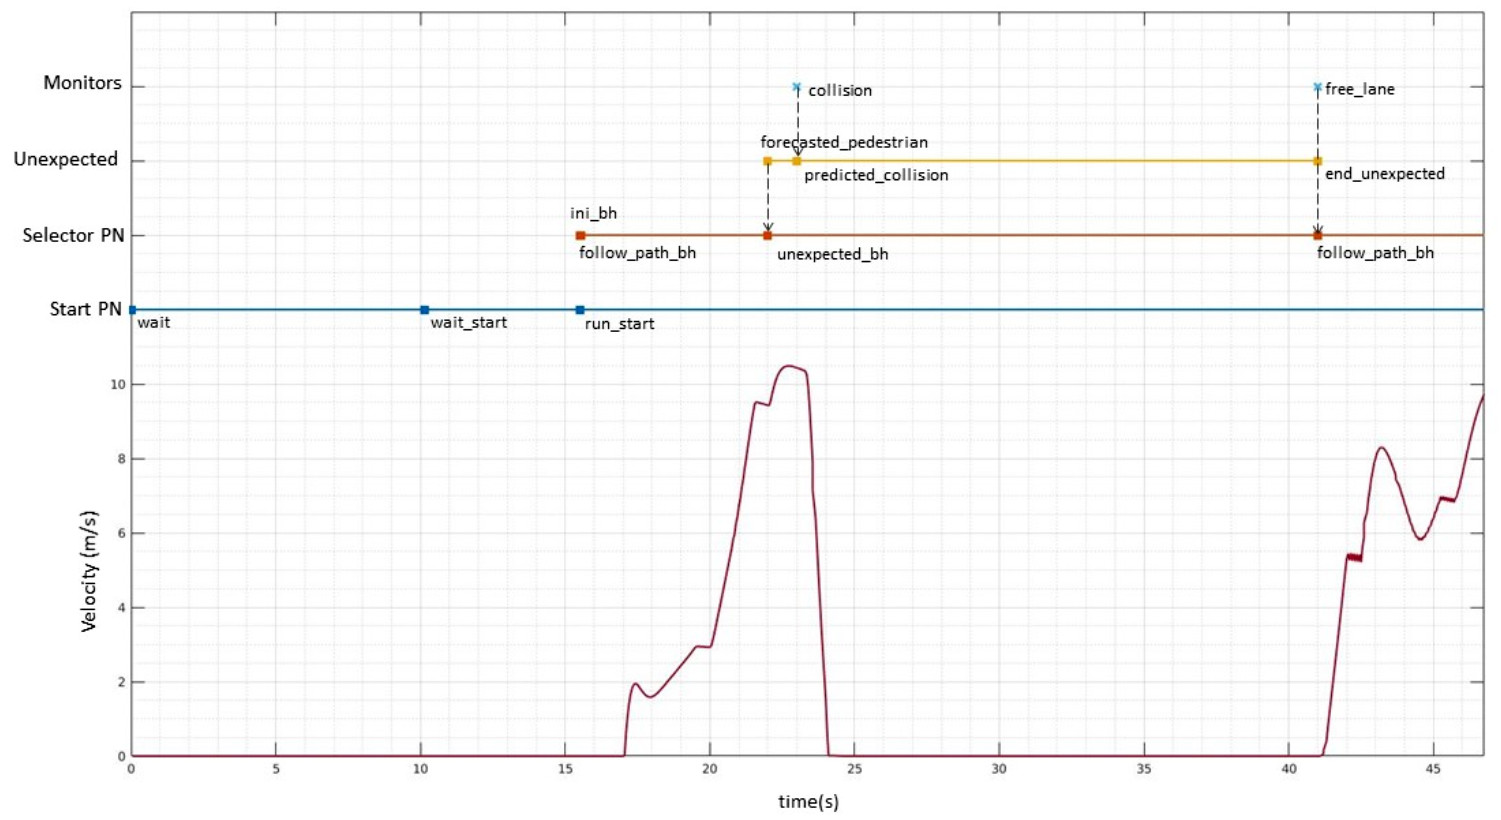
\includegraphics[width=0.8\textwidth]{chapter_4_SmartMOT/quantitative/unexpected_vru_temporal_graph.jpg}
	\caption[Unexpected Vulnerable Road User (VRU) temporal diagram]{Unexpected Vulnerable Road User (VRU) temporal diagram. At the top, the events produced by our monitors and map manager modules. In the middle, the selector, and start (background) PNs of our decision-making layer. At the bottom, the velocity of the car throughout the navigation}
	\label{fig:chapter_4_SmartMOT/quantitative/unexpected_vru_temporal_graph}
\end{figure}

In order to appreciate the behaviour of the vehicle during navigation, we incorporate a very illustrative temporal diagram (Figure \ref{fig:chapter_4_SmartMOT/unexpected_vru_temporal_graph}), representing a powerful manner to qualitatively validate how the architecture behaves in an end-to-end manner, since we can observe how the car behaves considering the different actions and events \cite{gomez2021train} provided by the executive layer, which is actually the output of the whole architecture before sending commands to the motor. As observed, the ego-vehicle starts far away from the adversary and starts its navigation. At second 22 a pedestrian that is in the sidewalk is detected, so tracking-by-detection and subsequent motion prediction must be carried as fast as possible to avoid collision, since the scenario is designed in such a way that the pedestrian must start walking in such a way the impact point (\(P_I\)) (Figure \ref{fig:chapter_4_SmartMOT/CPNA_scenario}) is in the center of the lane for each particular velocity. After that, our prediction module intersects the ego-vehicle forecasted trajectory and the pedestrian forecasted trajectory. If the Intersection over Union (IoU) is greater than a threshold (in this case, 0.01), a \textit{predictedcollision} flag is activated and the low-level (reactive) control, which always runs in the background of the decision-making layer, performs an emergency break until the car is stopped in front of the obstacle. Navigation is resumed once the obstacle leaves the driving lane. Table \ref{table:4_CPNA_results} compares the performance of the architecture by implementing \cite{gomez2020real} and a rectangular monitorized lane to retrieve the nearest object in route and predict collision against our proposal, where it can be appreciated that for velocities greater than 40 km/h, using HD map semantic and geometric information gives the car a valuable reaction time to anticipate the VRU behaviour and avoid the collision, achieving the highest score. 

\begin{table}[h]
	\centering
	\caption{Comparison of our two different perception strategies in the Car to Pedestrian Nearside Adult (CPNA) scenario. We bold the best score in \textbf{black}.}
	\label{table:4_CPNA_results}
	\begin{tabular}{c | c | c  c | c  c  } 
		\hline 
		\multicolumn{6}{c}{\textbf{CPNA}}\\
		\hline \hline
		\multirow{2}{*}{\textbf{\(v_{test}\)}} & \multirow{2}{*}{\textbf{\(score_{max}\)}} & \multicolumn{2}{c}{\textbf{Rectangular area + \cite{gomez2020real}}} & \multicolumn{2}{c}{\textbf{SmartMOT}} \\ 
		& & \(v_{impact}\) & \(score\) & \(v_{impact}\) & \(score\) \\
		\hline
		10 km/h & 1.00 & 0.0 km/h & 1.00 & 0.0 km/h & 1.00 \\
		20 km/h & 1.00 & 0.0 km/h & 1.00 & 0.0 km/h & 1.00 \\
		30 km/h & 2.00 & 0.0 km/h & 2.00 & 0.0 km/h & 2.00 \\
		40 km/h & 3.00 & 0.0 km/h & 3.00 & 0.0 km/h & 3.00 \\
		50 km/h & 2.00 & 23.82 km/h & 2.00 & 0.0 km/h & 2.00 \\
		60 km/h & 1.00 & 44.23 km/h & 0.00 & 0.0 km/h & 1.00  \\
		\hline \hline
		\textbf{Total} & 10.00 &  & 9.00 & & \textbf{10.0} \\
		\hline
	\end{tabular}
\end{table}

Figure \ref{fig:4_cpna_results} shows different analysis of the CPNA crash avoidance scenario with variable ego-vehicle and the incorporation of other traffic participants in the scenario (\ref{subfig:chapter_4_SmartMOT/euroncap_graphics_c} \ref{subig:chapter_4_SmartMOT/euroncap_graphics_d}). \(T_0\) corresponds with the moment the vehicle either stops or collides, and crosses \textbf{x} represent the moment in which the system sends a predicted collision signal to the executive layer, so it is coherent that crosses in tests where the ego-vehicle collides with the VRU are shifted to the right (prediction collision signal was given in time). Left column tracks all objects around the vehicle and adopts a geometric monitorized area to estimate the nearest distance and predicted collision, whilst right column uses HD map information to help in the Multi-Object Tracking and motion prediction tasks, monitoring only the most relevant traffic participants around the vehicle that is, the main purpose of SmartMOT.

As observed, using HD map information is able to avoid collision until a ego-vehicle velocity of 80 km/h, where SmartMOT is not able to send a signal of predicted collision (output of the system, as shown in Figure \ref{fig:chapter_4_SmartMOT/IV_2021}) in time, colliding at a velocity of 39.78 km/h. Nevertheless, this velocity at the moment of collision is even lower that the impact velocity (44.23 km/h) when testing the system under 60 km/h condition not using HD map in the MOT stage, illustrating how incorporating additional semantic and geometric map information helps the vehicle to react faster or at least mitigate the effect of collision. Moreover, we simulate both perception strategies using the most common velocities in urban scenarios, which range from 30 to 50 km/h, including \ref{subfig:chapter_4_SmartMOT/euroncap_graphics_c} \ref{fig:chapter_4_SmartMOT/euroncap_graphics_d} static adversaries (in particular, vehicles and pedestrians) which do not actually in the traffic scenario to fulfill the particular requirements stated by \cite{gutierrez2021validation} protocol. As expected, tracking all objects around the ego-vehicle and using the rectangular monitorized area suffers when the number of traffic participants is increased around the ego-vehicle, whilst SmartMOT holds this exponential increase by analyzing the objects and their corresponding role as relevant obstacles considering the information provided by the HD map, avoiding the collision in all situations.

\begin{figure}[h]
	\centering
	\begin{subfigure}{0.45\textwidth}
		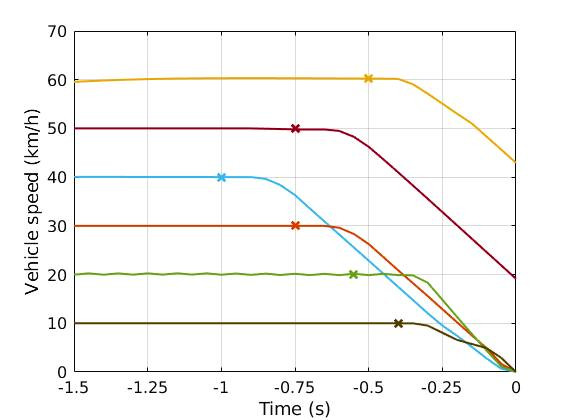
\includegraphics[width=\textwidth]{chapter_4_SmartMOT/quantitative/euroncap_without_adversaries_geometric.jpg}
		\caption{Rectangular monitored area without adversaries}
		\label{subfig:chapter_4_SmartMOT/euroncap_graphics_a}
	\end{subfigure}
	\hfill
	\begin{subfigure}{0.45\textwidth}
		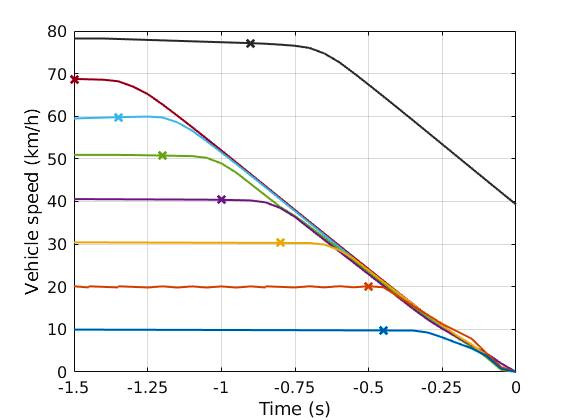
\includegraphics[width=\textwidth]{chapter_4_SmartMOT/quantitative/euroncap_without_adversaries_hdmap.jpg}
		\caption{SmartMOT area without adversaries}
		\label{subfig:chapter_4_SmartMOT/euroncap_graphics_b}
	\end{subfigure}
	\hfill
	\begin{subfigure}{0.45\textwidth}
		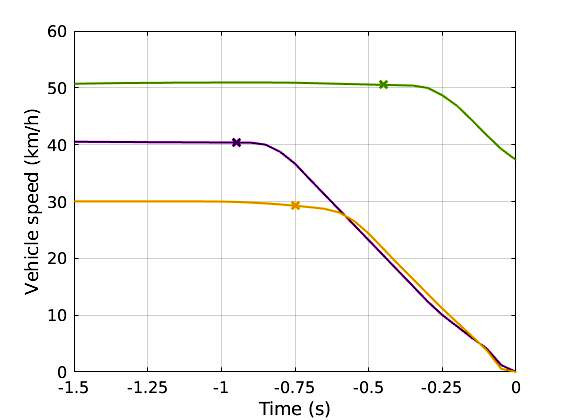
\includegraphics[width=\textwidth]{chapter_4_SmartMOT/quantitative/euroncap_with_adversaries_geometric.jpg}
		\caption{Rectangular monitored area with adversaries}
		\label{subfig:chapter_4_SmartMOT/euroncap_graphics_c}
	\end{subfigure}
	\hfill
	\begin{subfigure}{0.45\textwidth}
		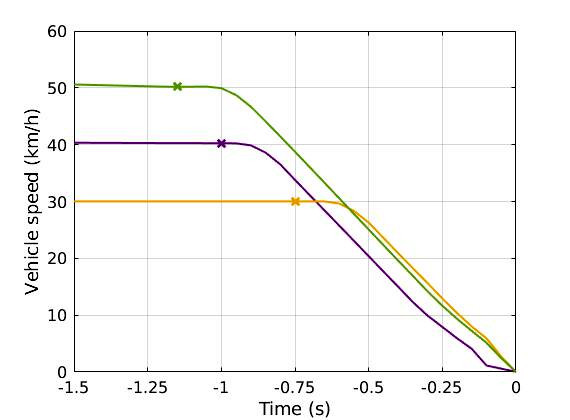
\includegraphics[width=\textwidth]{chapter_4_SmartMOT/quantitative/euroncap_with_adversaries_hdmap.jpg}
		\caption{SmartMOT area with adversaries}
		\label{subfig:chapter_4_SmartMOT/euroncap_graphics_d}
	\end{subfigure}
	
	\caption[Analysis of the Car to Pedestrian Nearside Adult (CPNA) crash avoidance scenario with variable ego-vehicle velocity]{Analysis of the Car to Pedestrian Nearside Adult (CPNA) crash avoidance scenario with variable ego-vehicle velocity. Left column (Figures \ref{subfig:subfig:chapter_4_SmartMOT/euroncap_graphics_a} and \ref{subfig:subfig:chapter_4_SmartMOT/euroncap_graphics_c}) adopts a rectangular monitorized area to estimate the nearest distance and predicted collision, Right column (Figures \ref{subfig:chapter_4_SmartMOT/euroncap_graphics_b} and \ref{subfig:chapter_4_SmartMOT/euroncap_graphics_d}) uses HD map information for this purpose. On the other hand, first row shows the scenario without additional traffic participants, second row analyzes the crash avoidance scenario including additional traffic participants to the road, monitorized sidewalk area and non-relevant sidewalk area. Crosses in the lines represent the moment in which the system sends a predicted collision signal to the executive layer}
	\label{fig:4_cpna_results}
\end{figure}

\section{Summary}
\label{sec:4_summary}

In this chapter we propose SmartMOT, a simple-yet-powerful pipeline that fuses the concepts of tracking-by-detection and HD map information to design a real-time and power-efficient Multi-Object Tracking (MOT) and Motion Prediction pipeline used to track and predict the future trajectories of only the most relevant obstacles around the ego-vehicle, incorporating a Monitored Lanes-based Attention Module to the pipeline, improving the way in which the vehicles are considered as relevant, and an additional module to evaluate different behavioural use cases and background behaviours. 

Then, experimental results focus on validating the tracking stage in the KITTI dataset. Once the best hyperparameters are obtain by means of an ablation study, an end-to-end validation of our pipeline in the Unexpected \ac{VRU} scenario is carried out, following an Euro-NCAP-based validation protocol, illustrating how integrating map information in the pipeline can minimize or at least reduce the impact velocity with the \ac{VRU} by reducing the computational complexity of the problem. Moreover, a temporal graph is depicted, representing a very intuitive and powerful manner to appreciate how the integration of this extended version of SmartMOT gives the vehicle a valuable time to anticipate the corresponding behaviours. We hope that our distributed pipeline can serve as a solid baseline on which others can build on to advance the state-of-the-art in fusing perception data and map information to perform real-time motion prediction and decision-making evaluation in arbitrarily complex urban scenarios. 